
% -----------------------------------------------------------------------------------
%      PACKAGES & OTHER DOCUMENT CONFIGURATIONS
% -----------------------------------------------------------------------------------
\documentclass[fontsize=11pt]{extarticle}

\usepackage[utf8]{inputenc}
\usepackage[T1]{fontenc}
\usepackage[british]{babel}
% ----------NEW BIBLATEX BIBLIOGRAPHY-----------------------------------------------
\usepackage[eprint=false,backend=bibtex,style = ieee]{biblatex} % Upgrades Bibliography Block Ragged helps break lines in url fixes error

\addbibresource{../BibFile.bib} %%% For biblatex
%e.g to add page number \footfullcite[chapter, p.~215]{AAIB}
% of \footnote{Footnote text goes here}
% This allows can use footfullcite commands
% Note urldate field must be in yyyy-mm-dd to work - use online type
% Remeber to use \printbibliography in the footer
% -----------------------------------------------------------------------------------
% \usepackage{sectsty}
\usepackage{url}

%%% --- The following two lines are what needs to be added --- %%%
\setcounter{biburllcpenalty}{7000}
\setcounter{biburlucpenalty}{8000}

\usepackage{amssymb,amsmath}
\numberwithin{figure}{section} %%%%% <<<<<< Puts Figure Numbering into Sections
\numberwithin{table}{section}%%%%% <<<<<< Puts Tables Numbering into Sections
\usepackage{ifxetex,ifluatex}  %<<<<<<<<< Edit FONT HERE
\ifnum 0\ifxetex 1\fi\ifluatex 1\fi=0 % if pdftex
  \usepackage[T1]{fontenc}
  \usepackage[utf8]{inputenc}
\else % if luatex or xelatex
  \ifxetex
    \usepackage{mathspec}
    \setmainfont[
 BoldFont={AvenirNext-Medium},ItalicFont={AvenirNext-Italic},
 BoldItalicFont={AvenirNext-MediumItalic}]{AvenirNext-Regular}
  \else
  % Font Package for XeLatex
    \usepackage{fontspec}
    \setmainfont{AvenirNext-Regular}
  \fi
  \defaultfontfeatures{Ligatures=TeX,Scale=MatchLowercase}
\fi
\usepackage[fit]{truncate} %Truncates headers that are too long
\usepackage[headheight=26pt,headsep=0.15cm]{geometry}
\usepackage{fancyhdr}
\usepackage{lastpage}
\usepackage{extramarks}
\usepackage{gensymb}
\usepackage{lipsum}
\usepackage{float}
\usepackage{graphicx}
\graphicspath{{../TempImg/}{../Img/}}%<<<<<<<<< Location of Template Images and Other Images, Add folders here
\usepackage{subfig}
\usepackage{wrapfig}
\usepackage[font ={small,it}]{caption}
\usepackage{amsfonts,amsthm} % Math packages
% \usepackage{cite}
\usepackage{csquotes}
%    \MakeAutoQuote{‘}{’}
%    \MakeAutoQuote*{“}{”} %corrects quote marks
\usepackage{enumitem} % resume numbered lists
\usepackage{multicol} %for mulitple colums in lists
\usepackage{booktabs} %<<<<<<<<< Table drawing package
\usepackage[table,xcdraw]{xcolor} %<<<<<<<<< Table drawing package
\usepackage{svg}
\usepackage{scrextend} %call footnotes
\usepackage[colorlinks, linkcolor = black, citecolor = black, filecolor = black, urlcolor = blue]{hyperref} % Creates Hyperlinks for references - add [colorlinks] for coloured hyperlinks
\usepackage{changepage} %Allows Adjust width to be used for the document (indenting paragraphs)
\usepackage{pdfpages} %Allows Pdfpages to be added to the document use \includepdf[pages={1}]{myfile.pdf}
\usepackage{pdflscape} %Change Pages from Portrait to Landscape
\usepackage{color,soul} %% Highlights text for markup
% \usepackage[compact]{titlesec}

\usepackage{pdfpages} %Allows Pdfpages to be added to the document use \includepdf[pages={1}]{myfile.pdf}
%%%%%%%For Condensed Report Format%%%%%%%%%%%%%%
\usepackage{titlesec}
\titlespacing\section{0pt}{6pt plus 2pt minus 2pt}{0pt plus 2pt minus 2pt}
\titlespacing\subsection{0pt}{0pt plus 3pt minus 2pt}{-3pt plus 2pt minus 2pt}
\titlespacing\subsubsection{0pt}{0pt plus 2pt minus 2pt}{-6pt plus 2pt minus 2pt}
\titlespacing\subsubsubsection{0pt}{-6pt plus 2pt minus 2pt}{-6pt plus 2pt minus 2pt}
\setlength{\multicolsep}{-1pt plus 2.0pt minus 1.5pt}% 50% of original values

% \titlespacing*{\section}{0pt}{1.1\baselineskip}{\baselineskip}

\renewcommand*{\thefootnote}{\alph{footnote}} %%% Changes footnotes to letters
\usepackage[bottom]{footmisc} %%% Pushes footnote to bottom and to the margin

\DeclareCiteCommand{\footcite}[\mkbibfootnote]
{\usebibmacro{cite:init}%
\usebibmacro{prenote}}
{\usebibmacro{citeindex}%
\printtext[brackets]{\usebibmacro{cite:comp}}}
{\multicitedelim}
{\usebibmacro{cite:dump}%
\usebibmacro{postnote}}

\newenvironment{indentpara}{\begin{adjustwidth}{2cm}{}}{\end{adjustwidth}} %Declare adjust width wiht indentpara
\renewcommand{\labelitemii}{$\circ$}
\renewcommand{\labelitemiii}{$\diamond$}
\renewcommand{\labelitemiii}{$\cdot$}

% -----------------------------------------------------------------------------------
%                 Code
% -----------------------------------------------------------------------------------
\usepackage{listings}
\lstset{inputpath=Code/}
\usepackage{color}
\definecolor{mygreen}{RGB}{28,172,0} % color values Red, Green, Blue
\definecolor{mylilas}{RGB}{170,55,241}

\lstset{language=Matlab,%
    %basicstyle=\color{red},
    breaklines=true,%
    basicstyle=\small,
    morekeywords={matlab2tikz},
    keywordstyle=\color{blue},%
    morekeywords=[2]{1}, keywordstyle=[2]{\color{black}},
    identifierstyle=\color{black},%
    stringstyle=\color{mylilas},
    commentstyle=\color{mygreen},%
    showstringspaces=false,%without this there will be a symbol in the places where there is a space
    numbers=left,%
    numberstyle={\tiny \color{black}},% size of the numbers
    numbersep=9pt, % this defines how far the numbers are from the text
    emph=[1]{for,end,break},emphstyle=[1]\color{red}, %some words to emphasise
    %emph=[2]{word1,word2}, emphstyle=[2]{style},
}

%% To Add Code Use :
% \lstinputlisting{myfun.m}
%% To input a file or :
% \begin{figure}[h]
% \begin{lstlisting}[language=Matlab]
% \end{lstlisting}
% \catpion{code}
% \end{figure}


% -----------------------------------------------------------------------------------
%                 Quotes
% -----------------------------------------------------------------------------------

\usepackage{epigraph}
% \epigraphsize{\small}% Default
\setlength\epigraphwidth{12cm}
\setlength\epigraphrule{0pt}

\usepackage{etoolbox}
\apptocmd{\sloppy}{\hbadness 10000\relax}{}{}%%%% > Removes Url bibliography warnings
\makeatletter
\patchcmd{\epigraph}{\@epitext{#1}}{\itshape\@epitext{#1}}{}{}
\makeatother

%%%% > For Quotes Use \epigraph{"Quote"}{ - \textup{Author}, Book}

% -----------------------------------------------------------------------------------
%                   NAMES & CLASS DEFINITION %<<<<<<<<< INSERT DETAILS HERE
% -----------------------------------------------------------------------------------

\newcommand{\ModuleTitle}{compgc22 Software Engineering}
\newcommand{\ModuleCode}{COMPGC22}

\newcommand{\AssignmentTitle}{DIY Tool Hire Service}
\newcommand{\University}{University College London}
\newcommand{\Faculty}{Faculty of Engineering Sciences}
\newcommand{\UniCrest}{TempImg/logoucl.png}
\newcommand{\UniLogo}{TempImg/logoucl.png}
\newcommand{\THS}{TempImg/logo.png}

\newcommand{\UniLogoHP}{TempImg/engLogo.jpg}%<<<<<<<<< Make Sure Files are in the Template
\newcommand{\StudentNameA}{Ahmed Afify}

\newcommand{\StudentNameB}{Gideon Acquaah-Harrison}

\newcommand{\StudentNameC}{Daiana Bassi}

\newcommand{\StudentNameD}{Antonio Manganelli}

\newcommand{\StudentNameE}{Cameron Mory}

\newcommand{\StudentNameF}{Stefan Poechhacker}

\newcommand{\StudentNameG}{Caroline Smith}

\newcommand{\StudentNameH}{Phoebe Staab}

\newcommand{\SupervisorNameA}{Rae Harbird}
\newcommand{\SupervisorEmailA}{r.harbird@ucl.ac.uk}



% -----------------------------------------------------------------------------------
%        PACKAGES FOR MARKDOWN CONVERSION - FOR USE If Using Markdown to Latex
% -----------------------------------------------------------------------------------
\usepackage{fixltx2e} % provides \textsubscript
% use upquote if available, for straight quotes in verbatim environments
\IfFileExists{upquote.sty}{\usepackage{upquote}}{}
% use microtype if available
\IfFileExists{microtype.sty}{%
\usepackage{microtype}
\UseMicrotypeSet[protrusion]{basicmath} % disable protrusion for tt fonts
}{}
\hypersetup{unicode=true,
            pdftitle={\AssignmentTitle},
            pdfauthor={\AssignmentTitle},
            pdfborder={0 0 0},
            breaklinks=true}
\urlstyle{same}  % don't use monospace font for urls
\usepackage{fancyvrb}
\VerbatimFootnotes % allows verbatim text in footnotes
\usepackage{longtable,booktabs}
\IfFileExists{parskip.sty}{%
\usepackage{parskip}
}{% else
\setlength{\parindent}{0pt}s
\setlength{\parskip}{6pt plus 2pt minus 1pt}
}
\setlength{\emergencystretch}{3em}  % prevent overfull lines
\providecommand{\tightlist}{%
  \setlength{\itemsep}{0pt}\setlength{\parskip}{0pt}}
% \setcounter{secnumdepth}{0}
% Redefines (sub)paragraphs to behave more like sections
\ifx\paragraph\undefined\else
\let\oldparagraph\paragraph
\renewcommand{\paragraph}[1]{\oldparagraph{#1}\mbox{}}
\fi
\ifx\subparagraph\undefined\else
\let\oldsubparagraph\subparagraph
\renewcommand{\subparagraph}[1]{\oldsubparagraph{#1}\mbox{}}
\fi

% -----------------------------------------------------------------------------------
%                   WORD COUTNER - for XeLaTex
% -----------------------------------------------------------------------------------
% \usepackage{xesearch}
% \newcounter{words}
% \newenvironment{counted}{%
%   \setcounter{words}{0}
%   \SearchList!{wordcount}{\stepcounter{words}}
%     {a?,b?,c?,d?,e?,f?,g?,h?,i?,j?,k?,l?,m?,
%     n?,o?,p?,q?,r?,s?,t?,u?,v?,w?,x?,y?,z?}
%   \UndoBoundary{'}
%   \SearchOrder{p;}}{%
%   \StopSearching}

% -----------------------------------------------------------------------------------
%                   MARGINS, HEADERS & FOOTERS
% -----------------------------------------------------------------------------------
 \geometry{
 left=25.4mm,
 right=25.4mm,
 top=25.4mm,
 bottom=25.4mm,
 }
\linespread{1.5}

\pagestyle{fancy}
\lhead{\includegraphics[width = 0.15\textwidth]{\UniLogo}}
% \chead{\AssignmentTitle}
\rhead{}
\lfoot{\AssignmentTitle}
\cfoot{}
\rfoot{Page \thepage} %%%% note the footer is swapped when page numbering style changes
\renewcommand\headrulewidth{0.4pt}
\renewcommand\footrulewidth{0.4pt}

\setlength\parindent{0pt}
 % \setlength{\headheight}{5mm}
\newcommand{\horrule}[1]{\rule{\linewidth}{#1}}

% -----------------------------------------------------------------------------------
%               DOCUMENT STRUCTURE COMMANDS
% -----------------------------------------------------------------------------------
% To sort out the formatting of header and footer when a page...
% ... split occurs "within" a problem environment.
\newcommand{\enterProblemHeader}[1]{
\nobreak\extramarks{#1 (Cont.)}\nobreak
\nobreak\extramarks{#1}{}\nobreak
}
% To sort out the formatting of header and footer when a page...
% ... split occur "between" problem environments.
\newcommand{\exitProblemHeader}[1]{
\nobreak\extramarks{#1 (Cont.)}\nobreak
\nobreak\extramarks{#1}{}\nobreak
}

% -----------------------------------------------------------------------------------
\begin{document}


%For PDF intro
% \includepdf[pages={-}]{DP4front.pdf}

  \setlength{\abovedisplayskip}{-18pt}
  \setlength{\belowdisplayskip}{0pt}
  \setlength{\abovedisplayshortskip}{-18pt}
  \setlength{\belowdisplayshortskip}{0pt}

  \setlist[enumerate]{itemsep=-2mm}
  \setlist[itemize]{itemsep=-2mm}


%----------------------------------------------------------------------------------------
                                  % TITLE PAGE FORMAT
%----------------------------------------------------------------------------------------
\pagenumbering{roman}
\begin{titlepage}

  \center % Center everything on the page
%----------------------------------------------------------------------------------------
% HEADING SECTION
%----------------------------------------------------------------------------------------
    \usefont{OT1}{bch}{b}{n}
    \normalfont \normalsize \textsc{\University} \\ [10pt]
    \normalfont \normalsize \textsc{\Faculty} \\ [25pt]
    
%----------------------------------------------------------------------------------------
% LOGO SECTION - Adds Univeristy Crest to the Report
%----------------------------------------------------------------------------------------
    % \includegraphics[width = 0.5\textwidth]{\UniLogoHP}\\[0.5cm]
    \includegraphics[width = 0.4\textwidth]{\UniCrest}\\[0.5cm]
    
%----------------------------------------------------------------------------------------
% HEADING SECTION
%----------------------------------------------------------------------------------------
    \normalfont \normalsize \textsc{\ModuleTitle} \\ [10pt]
%----------------------------------------------------------------------------------------
% TITLE SECTION
%----------------------------------------------------------------------------------------
    \horrule{0.5pt} \\[0.4cm]
    \includegraphics[width = 0.7\textwidth]{\THS}\\[0.5cm]
    % \huge \textbf{\AssignmentTitle} \\
    \horrule{2pt} \\[0.5cm]

%----------------------------------------------------------------------------------------
% AUTHOR SECTION
%----------------------------------------------------------------------------------------
\begin{minipage}{0.4\textwidth}
  \begin{flushleft} \large
  \emph{Supervisor:}\\
  % Change Name
  \textbf{\SupervisorNameA}\\
  % \textbf{\SupervisorNameB}
  \end{flushleft}
\end{minipage}\qquad
\begin{minipage}{0.4\textwidth}
  \begin{flushright} \large
  \emph{Email:} \\
  \SupervisorEmailA \\
  % \SupervisorEmailB
  \end{flushright}
\end{minipage} \\[1cm]
\begin{minipage}{0.4\textwidth}
  \begin{flushleft} \large
  \emph{Authors:} \\
    \textbf{\StudentNameA} \\
    \textbf{\StudentNameB} \\
    \textbf{\StudentNameC} \\
    \textbf{\StudentNameD}
  \end{flushleft}
\end{minipage}\qquad
\begin{minipage}{0.4\textwidth}
  \begin{flushright} \large
  \emph{ } \\
    \textbf{\StudentNameE} \\
    \textbf{\StudentNameF} \\
    \textbf{\StudentNameG} \\
    \textbf{\StudentNameH}
  \end{flushleft}
\end{minipage}\qquad


%----------------------------------------------------------------------------------------
% DATE SECTION
%----------------------------------------------------------------------------------------

\textit{{\large \today}}\\% Date, change the \today to a set date if you want to be precise

%----------------------------------------------------------------------------------------
% Disclaimer
%----------------------------------------------------------------------------------------
{\footnotesize This report is submitted as part requirement for the COMPGC22 module at UCL. It is substantially the result of our own work except where explicitly indicated in the text. The report may be freely copied and distributed provided the source is explicitly acknowledged.}

% ---------------------------------
\vfill % Fill the rest of the page with whitespace
\end{titlepage}

% \setcounter{page}{3}

\newpage


% -----------------------------------------------------------------------------------
%                                ABSTRACT
% -----------------------------------------------------------------------------------

\addcontentsline{toc}{section}{Abstract}
\begin{abstract}
  An abstract goes here.

\end{abstract}
\newpage

\addcontentsline{toc}{section}{Acknowledgements}
\section*{Acknowledgements}\label{acknowledgements}
The acknowledgement goes here.
\newpage
% -----------------------------------------------------------------------------------
%                              TABLE OF CONTENTS
% -----------------------------------------------------------------------------------

\tableofcontents
%
%
\newpage

\addcontentsline{toc}{section}{List of Tables}
\listoftables
\addcontentsline{toc}{section}{List of Figures}
\listoffigures

\newpage

\addcontentsline{toc}{section}{List of Acronyms}
\section*{List of Acronyms}\label{acronyms}
\textbf{CS}: Computer Science \\
\textbf{UCL}: Univeristy College London \\



\newpage

%% -----------------------------------------------------------------------------------
%%                              INTRODUCTION
%% -----------------------------------------------------------------------------------
\clearpage
\rfoot{Page \thepage}
\pagenumbering{arabic}
% \begin{counted} %<<<<<<<<<<<<<<STARTS WORD COUNTER
\hypertarget{project-overview}{%
\section{Project Overview}\label{project-overview}}

\hypertarget{team-members}{%
\subsection{Team Members}\label{team-members}}

\begin{table}[H]
      \centering
      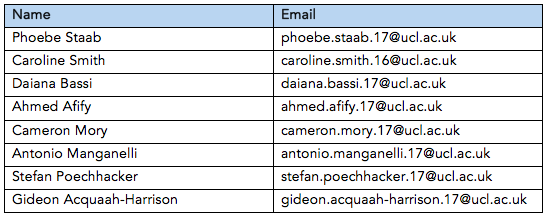
\includegraphics[trim = 0 0 0 0, clip, width=0.6\textwidth]{TempImg/teamtable.png}
      \caption{Team members and email addresses}
\label{conreq}
 \end{table}

\hypertarget{introduction}{%
\subsection{Introduction}\label{introduction}}

This report will elaborate on the process used by Group A to design the
DIY Tool Hire Service. The assignment was completed following the
use-case driven Unified Software Development Process (USDP){[}1{]}.

The iterative nature of the USDP resulted in multiple evolutions at
every step in the process. While each aspect of development -- from the
requirements gathering and use cases to the object-oriented diagrams --
underwent several iterations, only the final iterations have been
included within the report. All of the diagrams found in this report
were completed in Unified Modeling Language (UML) format, the industry
standard.

This chapter of the report will contain the problem statement, a
description of the scope of the project, a glossary of terms used
throughout the report, and a Gantt chart to display the project timeline
followed by the team. Following these sections is a summary of the
project management style. The subsequent chapters will cover the topics
of requirements gathering, use case development, object-oriented
analysis, and application mockups. Every stage of the development
process prior to the delivery of a minimum viable product (MVP) was
completed.

\hypertarget{problem-statement}{%
\subsection{Problem Statement}\label{problem-statement}}

These days, DIY home projects are very popular. Walk-throughs can be
found all over the internet for tasks such as making a bed-side table,
painting rooms with interesting patterns, or even building a shed.

One of the main problems when it comes to these tasks is that the
average person may not have the tools required readily available. It may
also be exceptionally expensive for people to go buy those tools as
well. Spending the money to purchase the tool is unlikely when it is
only needed for one specific project. DIY hobbyists require a service
that enables them to rent the tools they require for a much lower fee
than if they had to buy it themselves.

People who wish to complete home projects may also be limited by their
lack of experience with the tools. These people need to be provided with
advice and video tutorials that will show them how to properly use the
tools they wish to rent.

\hypertarget{project-scope}{%
\subsection{Project Scope}\label{project-scope}}

This report outlines the design process for a web application for
individuals who enjoy DIY projects but lack the tools to accomplish
them. The goal of the service is to provide a platform for people to
rent tools for short-term periods to complete their tasks. It will also
offer advice and tutorials for those who may require some help getting
started.

The central purpose of the web application is to allow individuals in
the London area to hire out tools for their projects. The customer will
be able to search through a selection of available tools, with the
ability to sort by type, name, or project. Having found the desired
tool, the customer will then check the calendar for its availability and
then add it to the basket. Upon check-out completion, the database will
be updated to reflect the dates for which the tool is booked to prevent
another customer from selecting those dates as well.

Customers may also view the blog containing weekly advice and subscribe
to it if they wish. They may also submit queries to the customer support
if they have any specific questions.

On the other side of the operation, employees may complete a range of
tasks including managing the tool listings, uploading new blog posts,
and responding to customer queries.

The success of the project would be measured by the delivery of the
completed stages of the software development process prior to the
creation of a prototype. This would include requirements gathering,
use-case analysis, object-oriented analysis and design models, and a
system mockup.

\hypertarget{project-glossary}{%
\subsection{Project Glossary}\label{project-glossary}}

In order to be clear and consistent throughout the project, specific
words and phrases were used. These can be found in the glossary below.

\begin{table}[H]
      \centering
      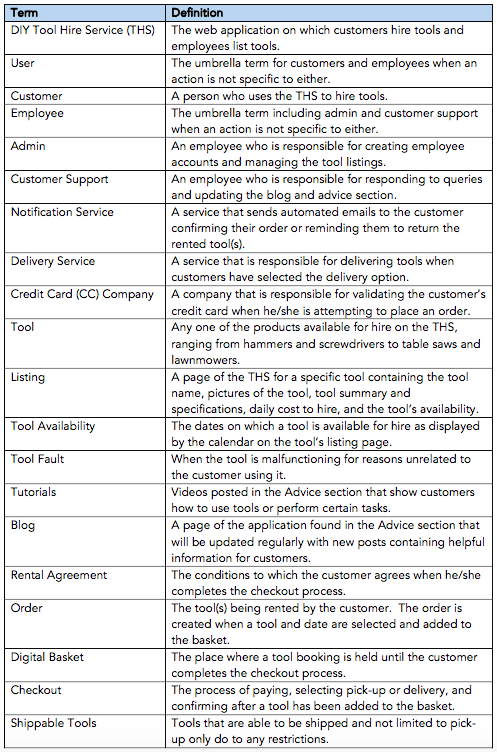
\includegraphics[trim = 0 0 0 0, clip, width=0.8\textwidth]{TempImg/glossary.png}
      \caption{Project glossary containing key terms}
\label{conreq}
 \end{table}

\hypertarget{gantt-chart}{%
\subsection{Gantt Chart}\label{gantt-chart}}

The Gantt charted shown below displays the project timeline followed by
the team.

\begin{figure}[H]
      \centering
      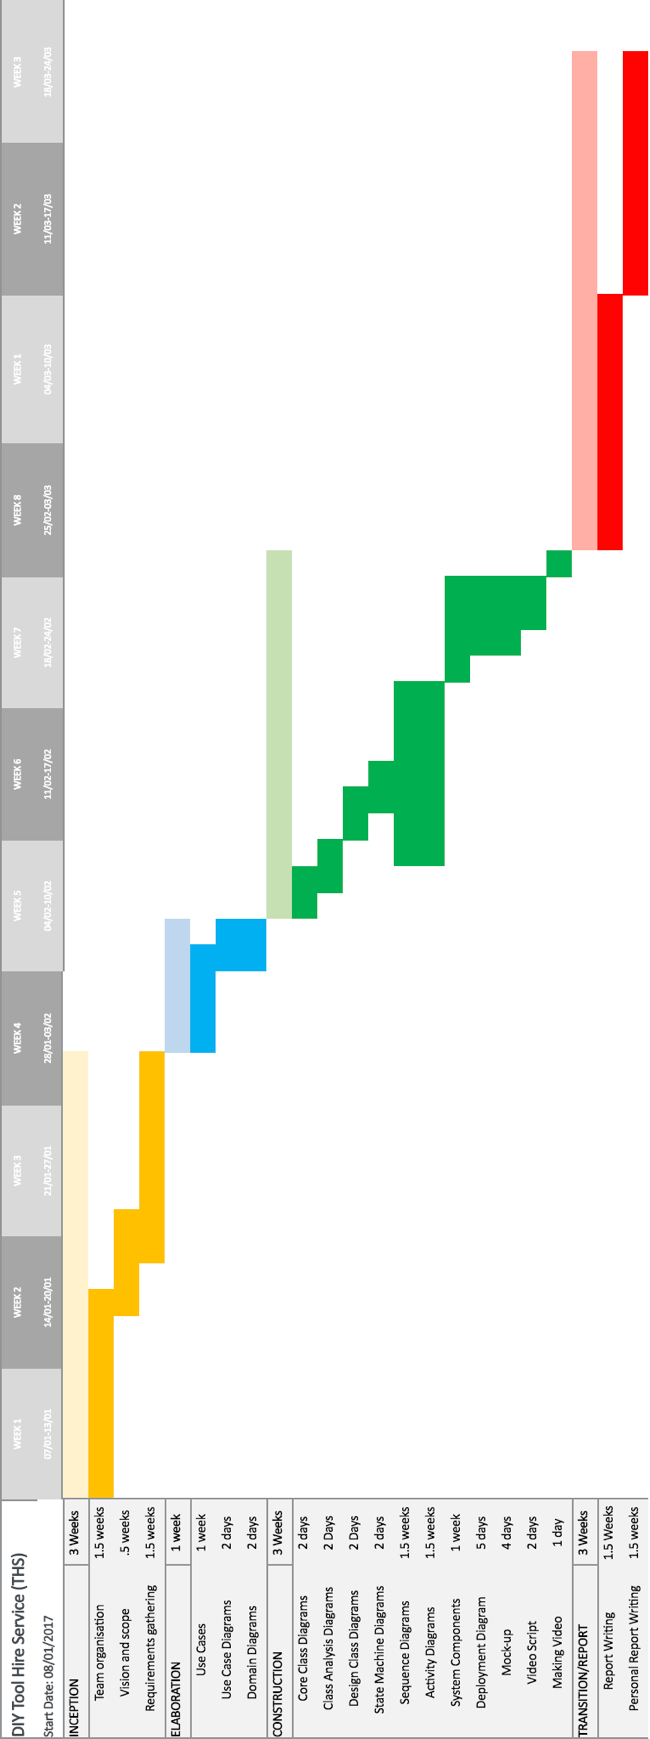
\includegraphics[trim = 0 0 0 0, clip, width=0.4\textwidth]{TempImg/gant.png}
      \caption{Gantt Chart Showing the Project Timeline}
 \end{figure}

\hypertarget{project-management-scrum-embedded-unified-process}{%
\subsection{Project Management: SCRUM Embedded Unified
Process}\label{project-management-scrum-embedded-unified-process}}

The Unified Process or UP was developed in the 1990s and is a pragmatic
and tested method for carrying out the development of a software system
and was designed specifically for use with UML. Essentially, it is a
process by which the who, what, and when of a development can be
determined. {[}2{]} The three main principles of the UP are:

\begin{itemize}
  \item The development process should be driven by use-cases and risk assessment
  \item Components related to the Warehouse management. It manages which tools are available and in which quantity.
  \item The development process should emphasize a quality system architectural model 
  \item Software should be developed via step-wise completion of subprojects and continuous refinement through iteration
\end{itemize}

Within each iteration, five workflows are explicitly defined by the UP.
These are requirements, analysis, design, implementation and testing.
(UP book) The broader project lifecycle is also covered in the UP and is
made up of four distinct phases which are inception, elaboration,
construction and transition. Within each of these phases, multiple
iterations should take place to suit the projects needs. Figure 1.2
illustrates how all of the elements of the UP are tied together into a
single project lifecycle.

\begin{figure}[H]
      \centering
      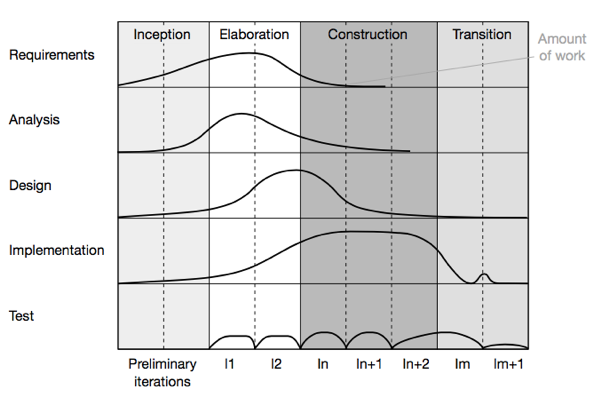
\includegraphics[trim = 0 0 0 0, clip, width=0.6\textwidth]{TempImg/UP.png}
      \caption{Outline of the Unified Process project lifecycle [2]}
 \end{figure}

SCRUM is a subset of Agile and is project management framework that grew
out of the failures of previous models such as the Waterfall model.
There are three empirical pillars that uphold any SCRUM project. {[}3{]}
These are:

\textbf{Transparency:} common standards are agreed upon within a team in
order to avoid ambiguity.

\textbf{Inspection:} Users must inspect and update SCRUM artifacts
throughout the development process.

\textbf{Adaptation:} Progress must be monitored by members of the SCRUM
team and if the process has deviated to an unacceptable extent, the
product(s) that resulted from that process must be reviewed and adapted.

These pillars underpin the SCRUM project lifecycle approach which
involves:

\begin{enumerate}
  \item The Scrum team meets in order to prioritize the artifacts in product backlog. This could be a list of required features for a product.
  \item Before a Sprint begins, the team has a Sprint planning meeting to decide what work will be done during the sprint.
  \item  The team does a backlog refinement to confirm that the project is still on track before beginning the Sprint to ensure that work will not be wasted.
  \item  During the 2-4 week Sprint, the team has daily meetings which are short, lasting only 15 minutes or less. 
  \item At the end of each sprint, the team members present their work and have a Sprint Retrospective to analyze what could be improved during the next sprint. [4]
\end{enumerate}

\begin{figure}[H]
      \centering
      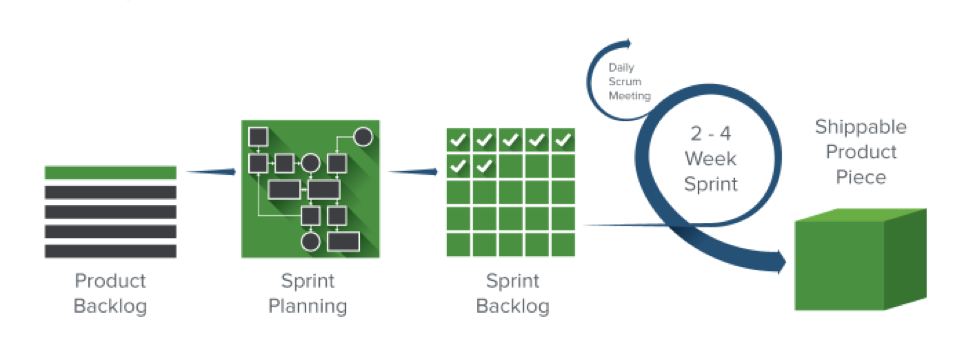
\includegraphics[trim = 0 0 0 0, clip, width=0.8\textwidth]{TempImg/SCRUM.png}
      \caption{The SCRUM project lifecycle [4]}
 \end{figure}

For the DIY THS project, the team utilized both of these methodologies
where they were suitable. The broader project lifecycle was shaped by
the tenants of the Unified process, while more day-to-day project
management was derived from some useful features of SCRUM.

The UP identifies that emphasizing system architecture and developing
based on use-cases leads to successful products. This was integral to
the development of the THS system. Given that the implementation was not
carried out for the THS, the team had the opportunity to rigorously
refine and identify essential use cases. From these use-cases, object
oriented (OO) UML models were derived. After the essential system
objectives were laid out through OO models, the architecture was
modeled. Additionally, the THS team made use of the four phases of the
Unified Process to help structure project progress which is illustrated
in the Gantt chart in Section 1.6.

While the team did not assign official SCRUM roles, certain useful
aspects of SCRUM were adopted. Early in the project, the team developed
a backlog of the tasks that needed to be accomplished throughout the
semester. Then, to fulfill these goals, the team worked in 1 week
Sprints followed by Retrospectives to assess the challenges encountered
in the previous week and plan the next Sprint. Additionally,
transparency and standardized communication was essential for such a
large group project and as such, a team glossary was used throughout.

Both the UP and SCRUM outline the importance of iteration, which was the
absolute core of the THS project. During the weekly Retrospectives,
analysis of the previous weeks work was done by the team members and the
project supervisor, which shed light on improvements to be made on the
current work products. In many cases, several Sprints were used to
refine a single work product.

Overall, the project management was more of an adaptation of key tenants
of both UP and SCRUM rather than an absolute adoption of all of their
aspects. Ultimately, being able to utilize aspects of such models to
suit the team's needs resulted in very smooth project coordination and
consistent progress throughout the semester.

\newpage

\hypertarget{requirements-gathering}{%
\section{Requirements Gathering}\label{requirements-gathering}}

\hypertarget{overview}{%
\subsection{Overview}\label{overview}}

The first task for this project was to develop a list of requirements
for the DIY Tool Hire Service. To do so, the team began by organizing a
meeting to discuss the scope of the project. Once everyone came to a
mutual understanding, the process of coming up with the requirements
began. During the meeting, the team reviewed the needs of the customer
when using this type of service. Each member then continued to develop
requirements individually by researching existing web sites to find
important functionalities as well as areas which may be improved.

This initial period of requirements development involved a lot of
brainstorming. The aim was to create a list of requirements that fully
encompassed the website's functionalities. This would save time and
effort further down the line, as making up for mistakes made during the
requirement gathering period can become extremely costly {[}5{]}.

The importance of the requirements gathering stage in the overall scope
of the project cannot be overstated. The requirements play a pivotal
role in the progression of the project, directly influencing the
development of use cases. The use cases then go on to influence the
classes and methods used, which in turn influence many of the future
diagrams. With that in mind, it was very important that the requirements
gathering was done correctly. This is reflected in the significant
portion of time that was allotted to develop the requirements, as seen
in the Gantt chart in Section 1.6.

\hypertarget{requirements}{%
\subsection{Requirements}\label{requirements}}

Although initially long and containing duplicates, the list of
requirements was refined to fall in line with the scope of the project.
These requirements were then broken down into subsections such as ``Tool
Hiring Process'' and ``Help \& Advice'' to aid in navigating the list
and ensuring the user's needs were accounted for. In Table 2.1, all of
the functional and non-functional requirements have been assigned IDs
and descriptions, as well as indications about the type of activity and
the actors involved. Additionally, every requirement was given a level
of priority utilizing the MoSCoW system {[}6{]}.

\begin{table}[H]
      \centering
      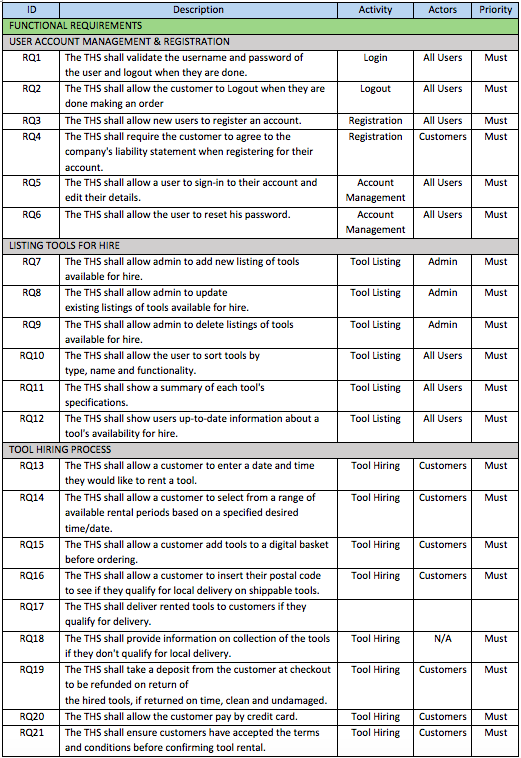
\includegraphics[trim = 0 0 0 0, clip, width=0.9\textwidth]{TempImg/req1.png}
 \end{table}

\begin{table}[H]
      \centering
      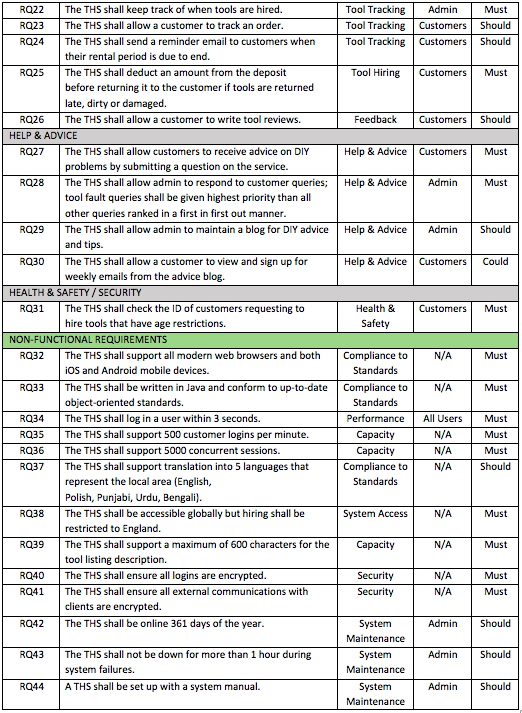
\includegraphics[trim = 0 0 0 0, clip, width=0.9\textwidth]{TempImg/req2.png}
      \caption{MoSCoW prioritization of requirements for the THS system}
 \end{table}

\hypertarget{domain-model-diagram}{%
\subsection{Domain Model Diagram}\label{domain-model-diagram}}

The domain model is used to represent the real-world actors and
entities, as well as the relationships between them in the context of
the problem space. It is a static model, in that it does not show any
time or information flow. To develop the diagram, the actors and
entities were derived from the requirements list, with nouns becoming
entities and verbs becoming relationships. They were then used to help
reduce ambiguities that may arise during the design period as well as
managing the complexity {[}7{]}. Additionally, the actors and entities
represented some possible classes for the later stages of the
development.

The domain model diagram was finalized over a sequence of iterations,
with the latest version seen in Figure 2.1 below. The actors, entities,
and relationships between them are shown using UML notation. Once the
entities were known, it was easier to construct the use cases more
effectively.

\begin{figure}[H]
      \centering
      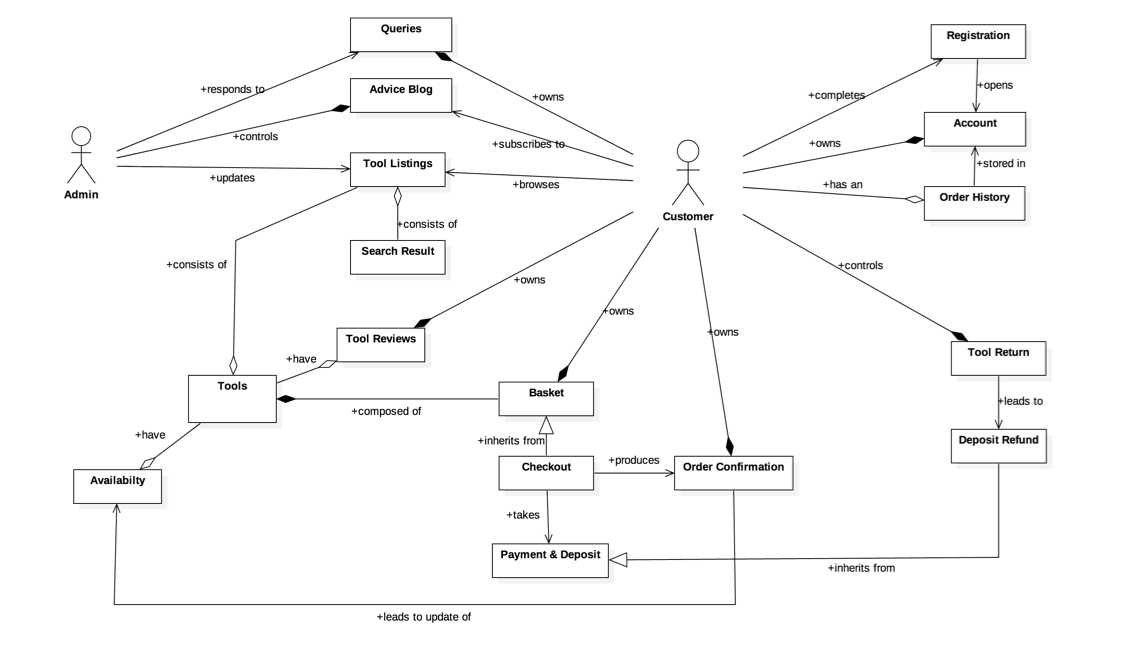
\includegraphics[trim = 0 0 0 0, clip, width=0.99\textwidth]{TempImg/domain.png}
      \caption{Domain model diagram}
 \end{figure}

\newpage

\hypertarget{use-cases}{%
\section{Use Cases}\label{use-cases}}

\hypertarget{overview-1}{%
\subsection{Overview}\label{overview-1}}

Having finished with the requirements gathering stage, the next task in
the process involved developing and analysing a list of use cases. Each
use case represents some interaction taking place between an actor and
the DIY Tool Hire Service {[}8{]}.

The use case analysis stage is essential to the development of a proper
software system. It is vital that each of the requirements listed in
Table 2.1 is accounted for when creating the use cases. This was
accomplished using an iterative process, during which the requirements
were expanded and modified, and the use cases were adapted to support
those changes.

During the use case analysis period, the team completed the use case
list, use case diagram, use case specifications, and the use
case/requirements matrix. These tables and figures are found in the
following subsections of this chapter.

\hypertarget{use-case-listing}{%
\subsection{Use Case Listing}\label{use-case-listing}}

When brainstorming the potential list of use cases, it was necessary for
the team to determine who the actors would be when interacting with the
DIY Tool Hire Service. The list of actors that was decided on based on
the requirements came to: Customer, Admin, Credit Card Company,
Notification Service, Customer Support, Database, and Delivery Service.
With the requirements and these actors in mind, a list of use cases was
established. Over the course of several iterations, the list was adapted
until the final list below was developed.

\begin{table}[H]
      \centering
      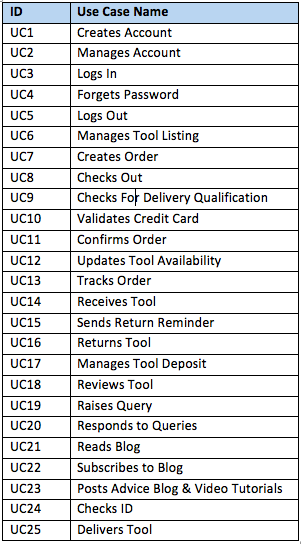
\includegraphics[trim = 0 0 0 0, clip, width=0.5\textwidth]{TempImg/UCListing.png}
      \caption{Use case listing}
 \end{table}

\hypertarget{use-case-diagram}{%
\subsection{Use Case Diagram}\label{use-case-diagram}}

The use case listing from above was translated into a use case diagram.
The diagram presents the use cases in a more clearly illustrated manner.
The team utilized the \textless{}\textgreater{} relationship as a way to
add optional behaviours to certain use cases, as well as the
\textless{}\textgreater{} relationship to simplify larger use cases into
more manageable parts {[}9{]}.

\begin{figure}[H]
      \centering
      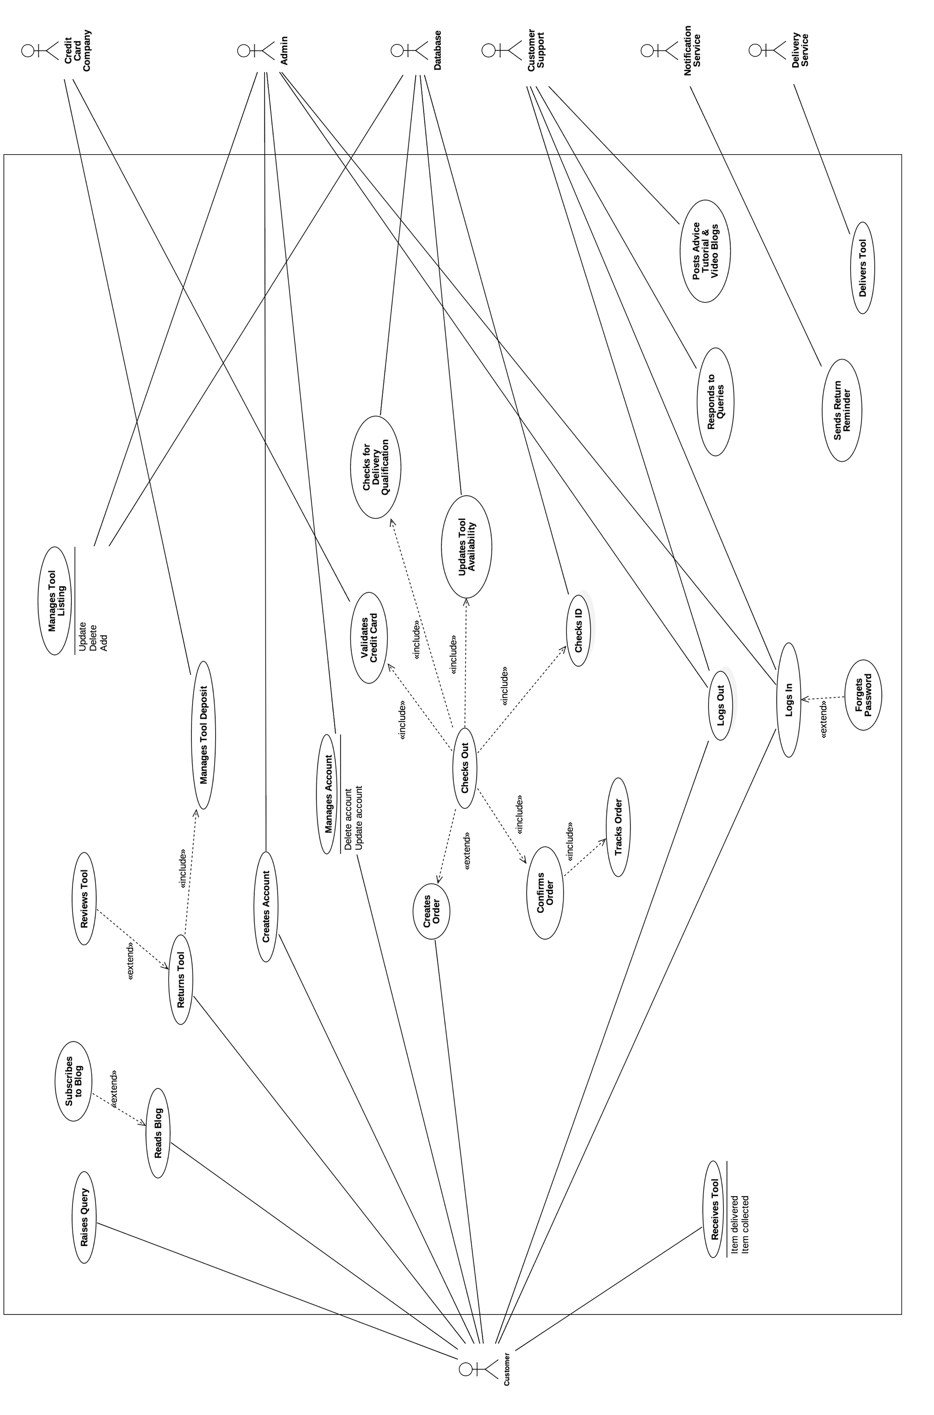
\includegraphics[trim = 0 0 0 0, clip, width=0.9\textwidth]{TempImg/UCDiagram.png}
      \caption{Use case diagram}
 \end{figure}

\hypertarget{use-case-specifications}{%
\subsection{Use Case Specifications}\label{use-case-specifications}}

Continuing the development process, the team took the use cases depicted
above and provided a much more detailed information for each including a
description, the actors involved, pre- and post-conditions, as well as
the main and alternative flows. As the use case specifications were
written, further alterations took place with the list of use cases. The
list of use cases was refined, and the specifications continuously
updated throughout the project as more thought went into the behaviours
of the actors. The following specifications for the finalized list of
use cases played a key role in the upcoming design period of the project
{[}8{]}.

\begin{figure}[H]
      \centering
      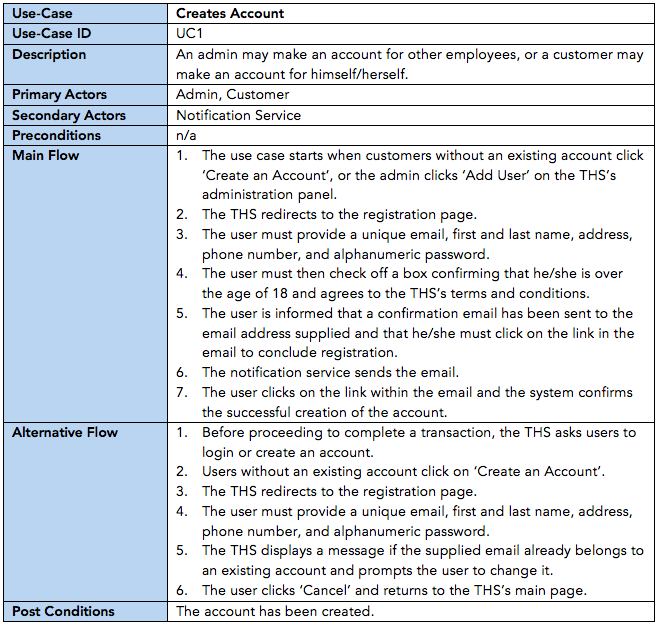
\includegraphics[trim = 0 0 0 0, clip, width=0.7\textwidth]{TempImg/UC1.png}
 \end{figure}

\begin{figure}[H]
      \centering
      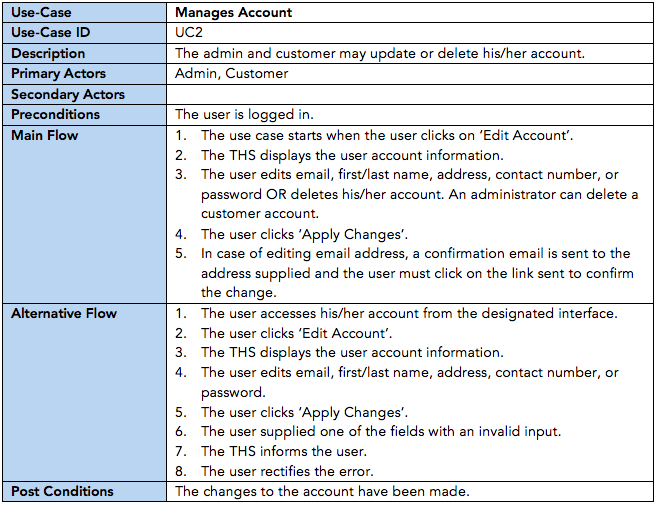
\includegraphics[trim = 0 0 0 0, clip, width=0.7\textwidth]{TempImg/UC2.png}
 \end{figure}

\begin{figure}[H]
      \centering
      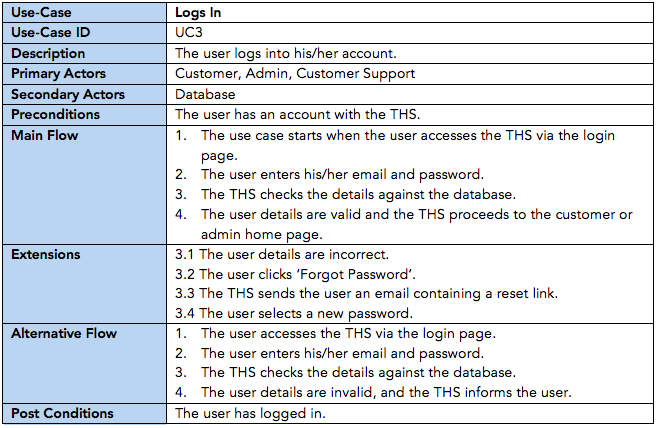
\includegraphics[trim = 0 0 0 0, clip, width=0.7\textwidth]{TempImg/UC3.png}
 \end{figure}

\begin{figure}[H]
      \centering
      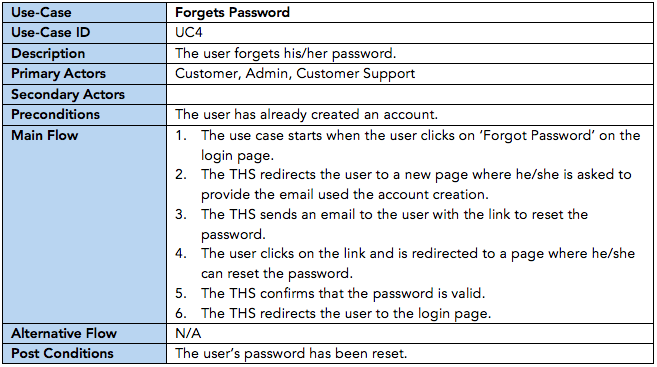
\includegraphics[trim = 0 0 0 0, clip, width=0.7\textwidth]{TempImg/UC4.png}
 \end{figure}

\begin{figure}[H]
      \centering
      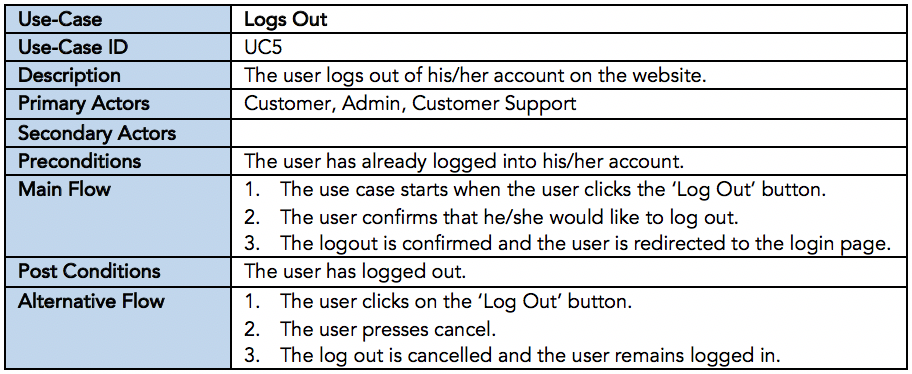
\includegraphics[trim = 0 0 0 0, clip, width=0.7\textwidth]{TempImg/UC5.png}
 \end{figure}

\begin{figure}[H]
      \centering
      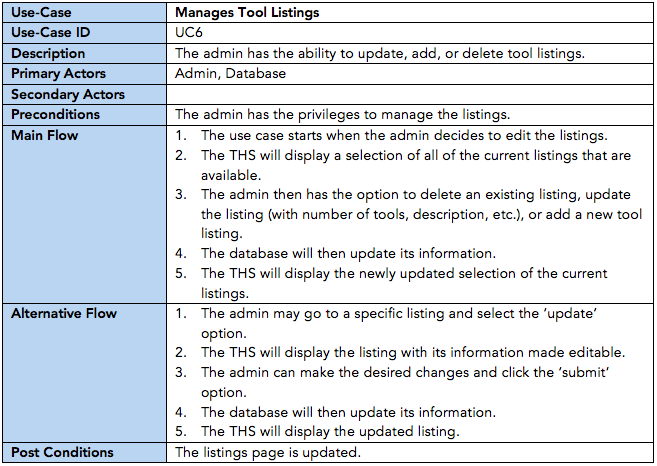
\includegraphics[trim = 0 0 0 0, clip, width=0.7\textwidth]{TempImg/UC6.png}
 \end{figure}

\begin{figure}[H]
      \centering
      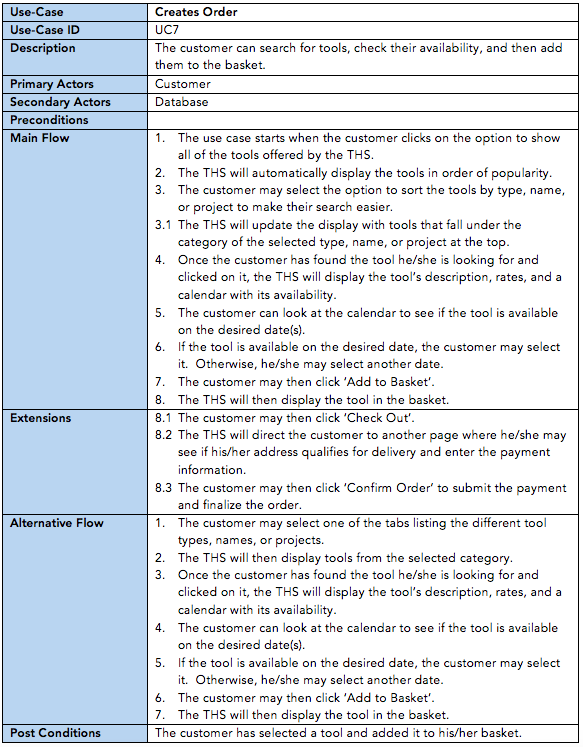
\includegraphics[trim = 0 0 0 0, clip, width=0.7\textwidth]{TempImg/UC7.png}
 \end{figure}

\begin{figure}[H]
      \centering
      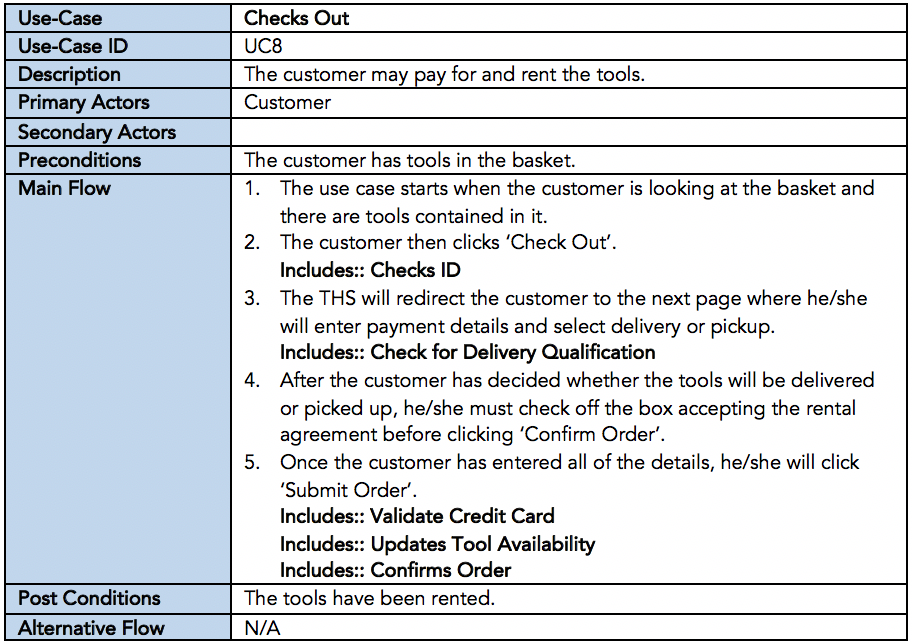
\includegraphics[trim = 0 0 0 0, clip, width=0.7\textwidth]{TempImg/UC8.png}
 \end{figure}

\begin{figure}[H]
      \centering
      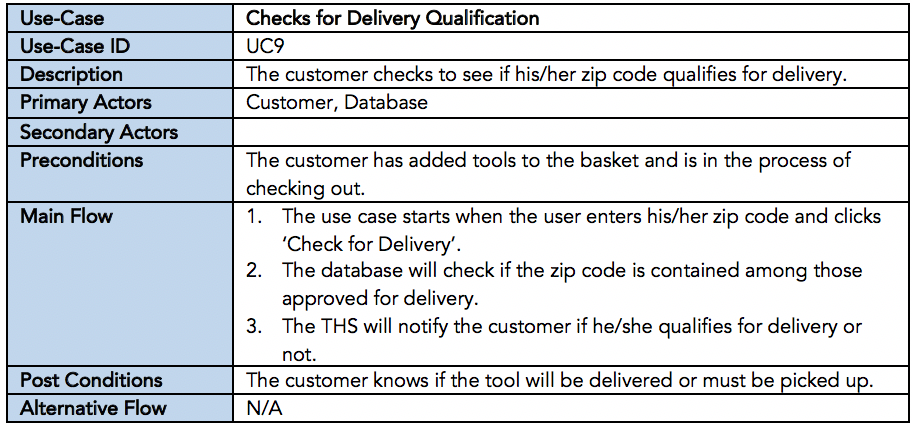
\includegraphics[trim = 0 0 0 0, clip, width=0.7\textwidth]{TempImg/UC9.png}
 \end{figure}

\begin{figure}[H]
      \centering
      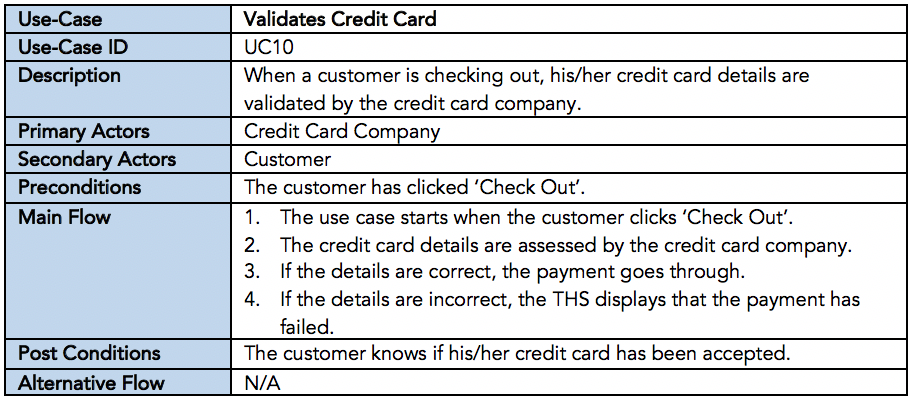
\includegraphics[trim = 0 0 0 0, clip, width=0.7\textwidth]{TempImg/UC10.png}
 \end{figure}

\begin{figure}[H]
      \centering
      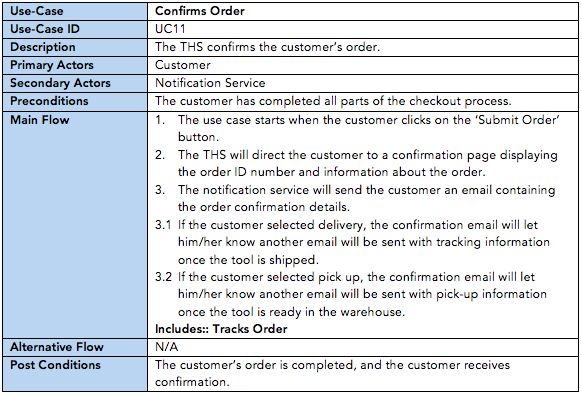
\includegraphics[trim = 0 0 0 0, clip, width=0.7\textwidth]{TempImg/UC11.png}
 \end{figure}

\begin{figure}[H]
      \centering
      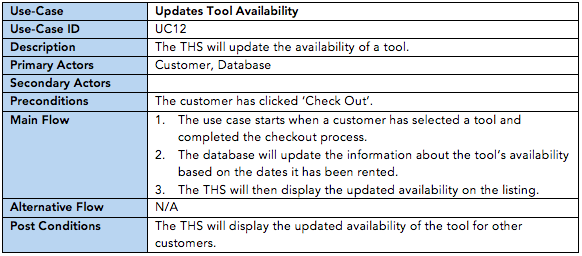
\includegraphics[trim = 0 0 0 0, clip, width=0.7\textwidth]{TempImg/UC12.png}
 \end{figure}

\begin{figure}[H]
      \centering
      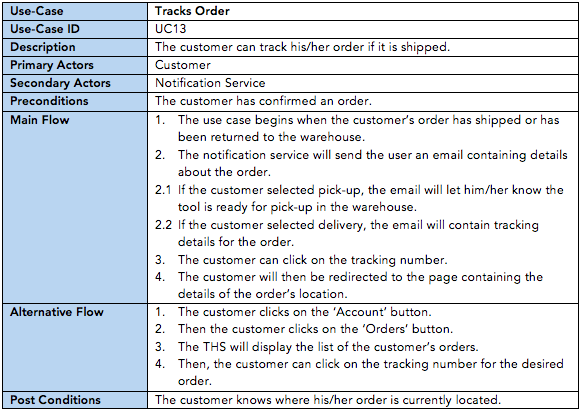
\includegraphics[trim = 0 0 0 0, clip, width=0.7\textwidth]{TempImg/UC13.png}
 \end{figure}

\begin{figure}[H]
      \centering
      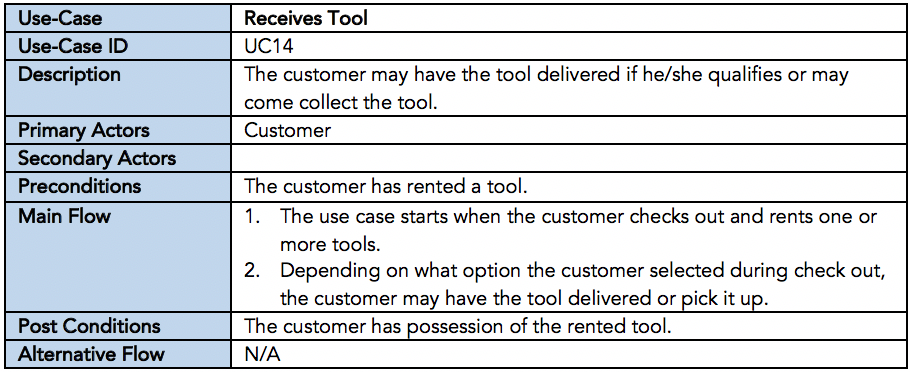
\includegraphics[trim = 0 0 0 0, clip, width=0.7\textwidth]{TempImg/UC14.png}
 \end{figure}

\begin{figure}[H]
      \centering
      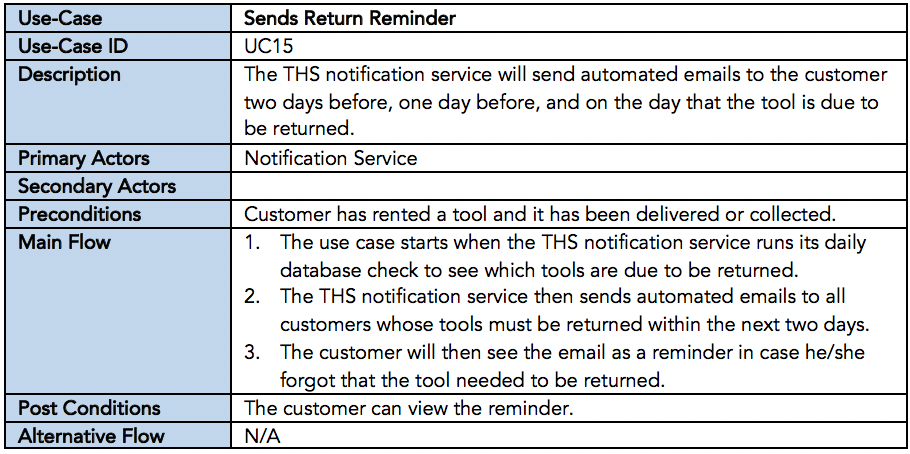
\includegraphics[trim = 0 0 0 0, clip, width=0.7\textwidth]{TempImg/UC15.png}
 \end{figure}

\begin{figure}[H]
      \centering
      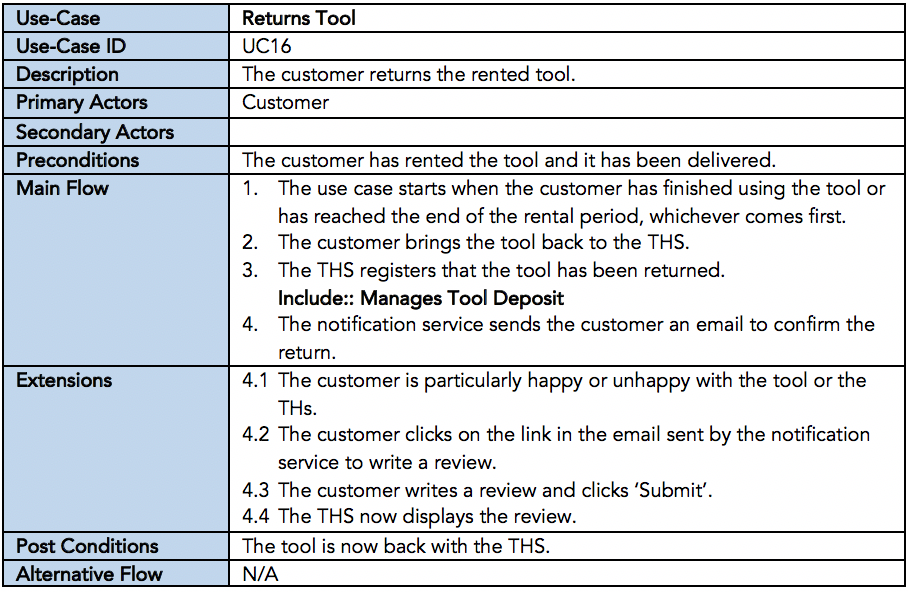
\includegraphics[trim = 0 0 0 0, clip, width=0.7\textwidth]{TempImg/UC16.png}
 \end{figure}

\begin{figure}[H]
      \centering
      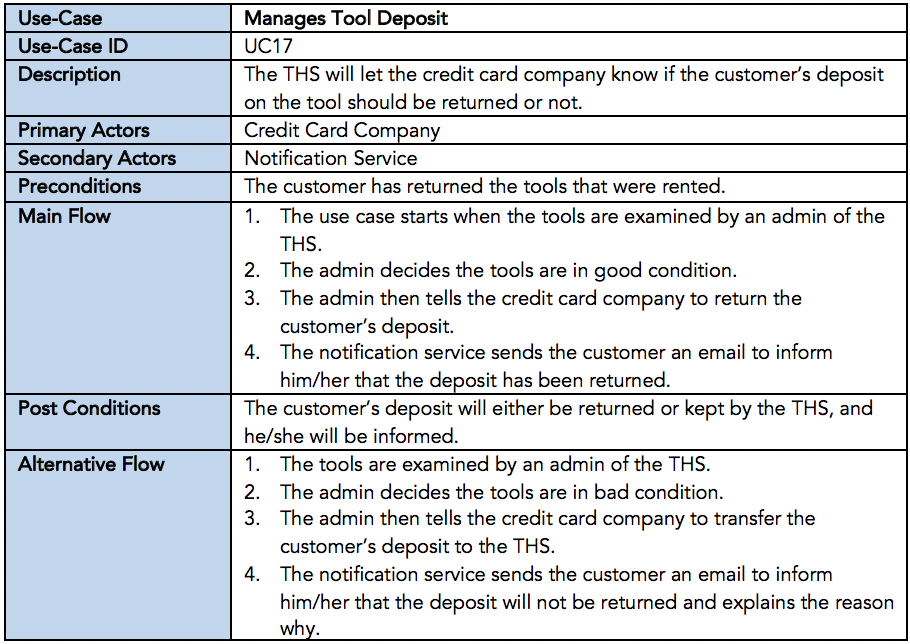
\includegraphics[trim = 0 0 0 0, clip, width=0.7\textwidth]{TempImg/UC17.png}
 \end{figure}

\begin{figure}[H]
      \centering
      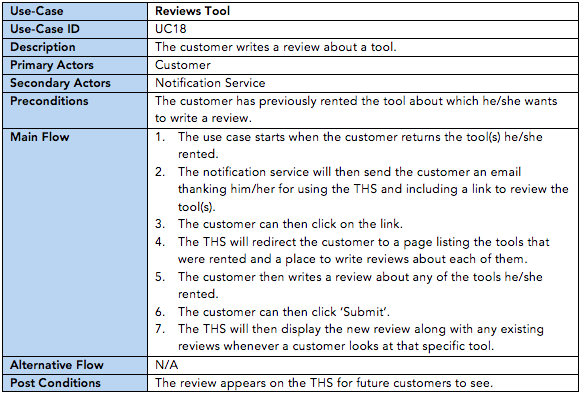
\includegraphics[trim = 0 0 0 0, clip, width=0.7\textwidth]{TempImg/UC18.png}
 \end{figure}

\begin{figure}[H]
      \centering
      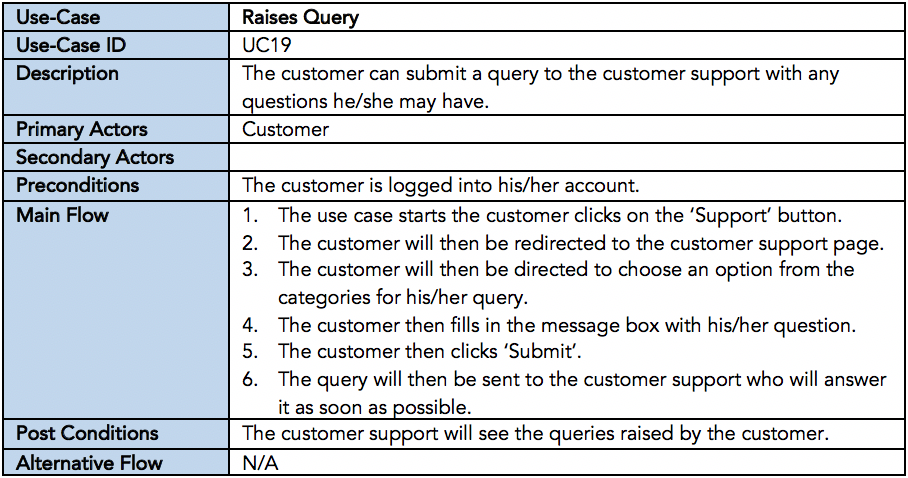
\includegraphics[trim = 0 0 0 0, clip, width=0.7\textwidth]{TempImg/UC19.png}
 \end{figure}

\begin{figure}[H]
      \centering
      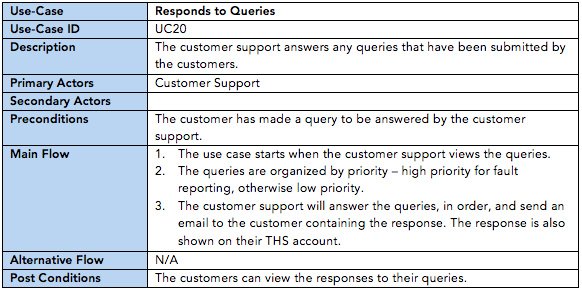
\includegraphics[trim = 0 0 0 0, clip, width=0.7\textwidth]{TempImg/UC20.png}
 \end{figure}

\begin{figure}[H]
      \centering
      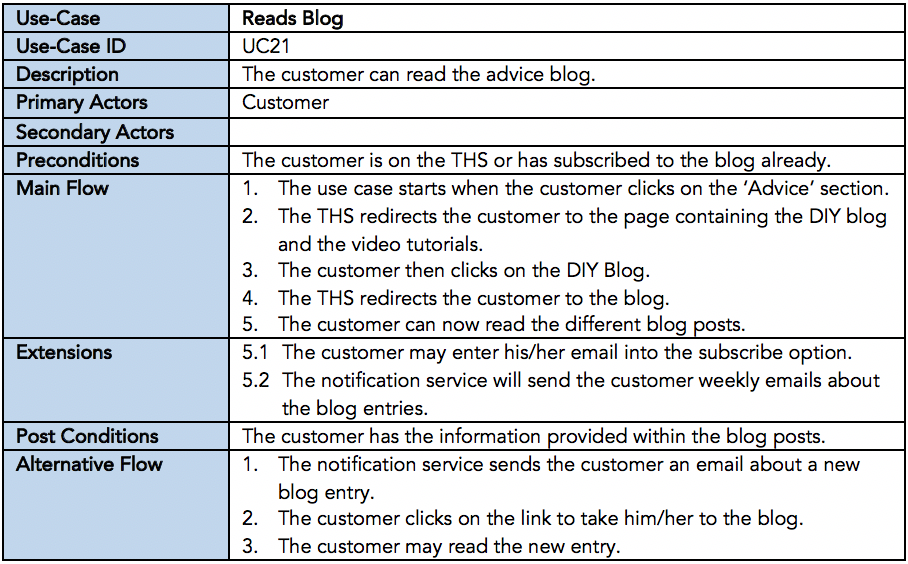
\includegraphics[trim = 0 0 0 0, clip, width=0.7\textwidth]{TempImg/UC21.png}
 \end{figure}

\begin{figure}[H]
      \centering
      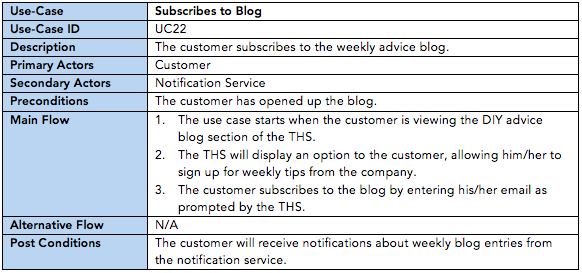
\includegraphics[trim = 0 0 0 0, clip, width=0.7\textwidth]{TempImg/UC22.png}
 \end{figure}

\begin{figure}[H]
      \centering
      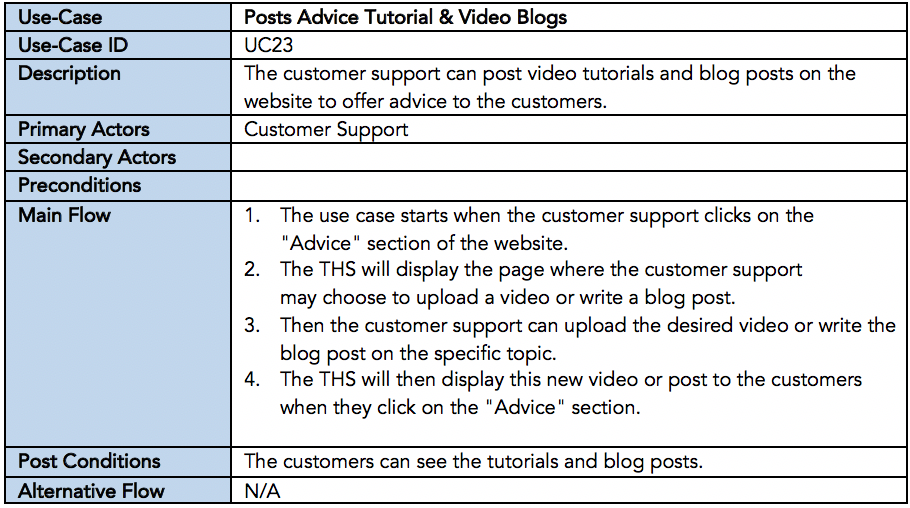
\includegraphics[trim = 0 0 0 0, clip, width=0.7\textwidth]{TempImg/UC23.png}
 \end{figure}

\begin{figure}[H]
      \centering
      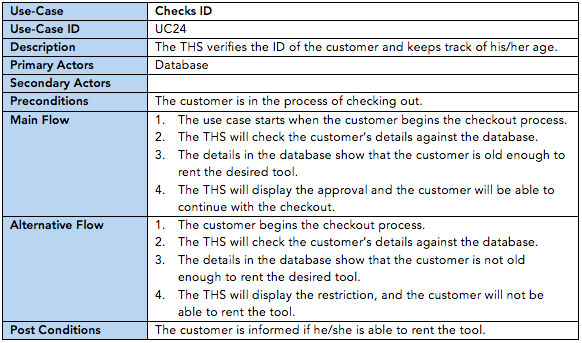
\includegraphics[trim = 0 0 0 0, clip, width=0.7\textwidth]{TempImg/UC24.png}
 \end{figure}

\begin{figure}[H]
      \centering
      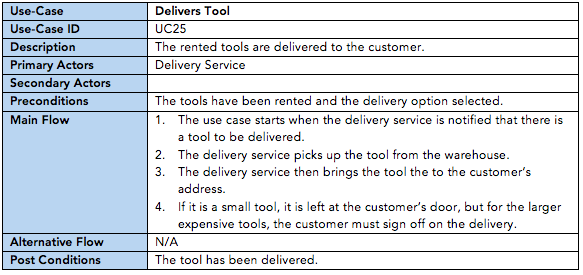
\includegraphics[trim = 0 0 0 0, clip, width=0.7\textwidth]{TempImg/UC25.png}
 \end{figure}

\newpage

\hypertarget{use-caserequirements-matrix}{%
\subsection{Use Case/Requirements
Matrix}\label{use-caserequirements-matrix}}

The last task to accomplish during the use case analysis stage was to
create a use case/requirements matrix. This matrix, which displays the
requirements on the left side and the use cases across the top, is
intended to confirm that each of the requirements is being satisfied by
one of the use cases and that each use case serves the purpose of
meeting a requirement {[}4{]}. As seen below, the requirements and use
cases established by the team satisfy these conditions.

\begin{figure}[H]
      \centering
      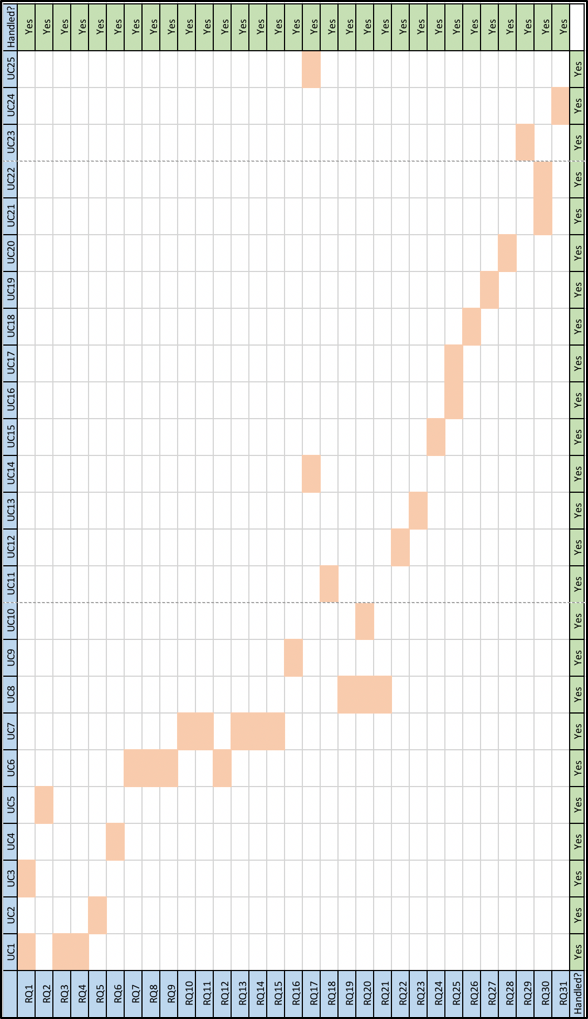
\includegraphics[trim = 0 0 0 0, clip, width=0.55\textwidth]{TempImg/UCRMatrix.png}
      \caption{Use case/Requirements matrix to describe how use cases fulfill system requirements}
 \end{figure}

\hypertarget{object-oriented-analysis-and-design}{%
\section{Object-Oriented Analysis and
Design}\label{object-oriented-analysis-and-design}}

\hypertarget{activity-diagrams}{%
\subsection{Activity diagrams}\label{activity-diagrams}}

Activity diagrams help to model system processes through a series of
activities. They have convenient notation, similar to flow charts and
can be thought of as Object Oriented flowcharts. {[}9{]} Unlike in class
diagrams or sequence diagrams, actions are written in plain English as
these diagrams serve as predecessors to more complex, class-oriented
models.

The THS team used activity diagrams to model complete processes
including both software and real-world activities, and in doing so
indicated the relationship between such activities and how they are
carried out to fulfill system requirements. Included in these
representations are start and stop states, indicating the beginning and
end of an activity and forks and joins, to illustrate when activity
states occur concurrently. {[}9{]} Alternative flows are modeled by
decisions, represented by a diamond, and indicate different directions
that can be taked based on a certain condition. The final iterations of
activity diagrams for the THS are shown below as well as a key to
activity diagram syntax.

\begin{figure}[H]
      \centering
      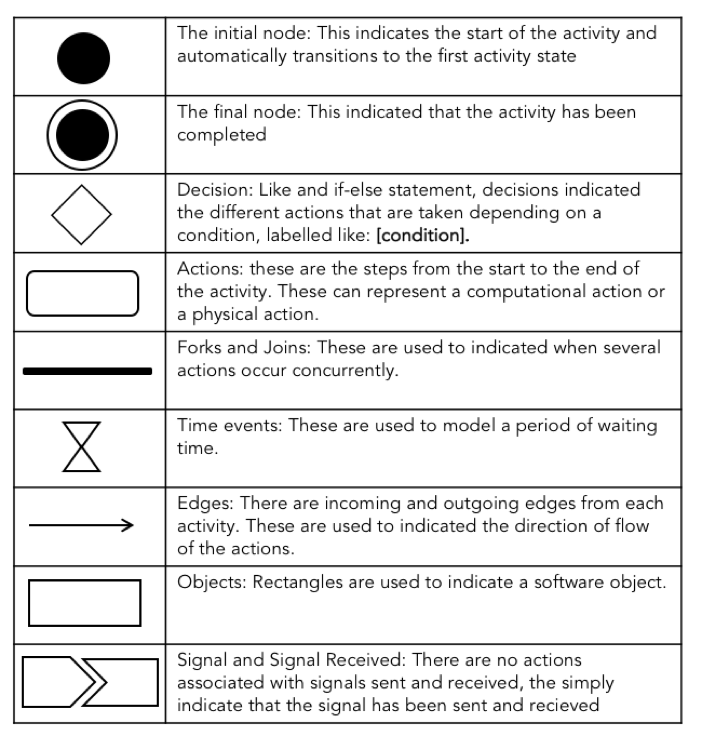
\includegraphics[trim = 0 0 0 0, clip, width=0.6\textwidth]{TempImg/ADKey.png}
      \caption{Key for activity diagram symbols}
 \end{figure}

\begin{figure}[H]
      \centering
      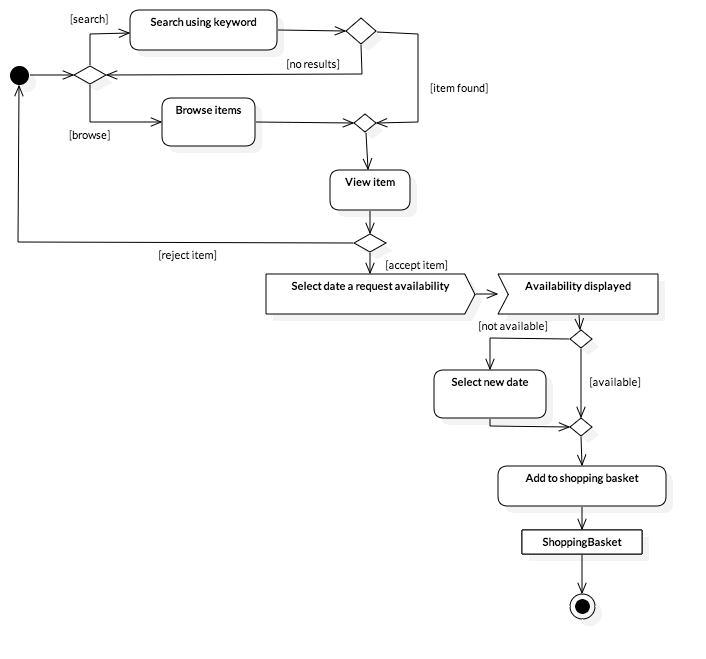
\includegraphics[trim = 0 0 0 0, clip, width=0.65\textwidth]{TempImg/makeOrderAD.png}
      \caption{Activity diagram for UC7:Creates Order}
 \end{figure}

\begin{figure}[H]
      \centering
      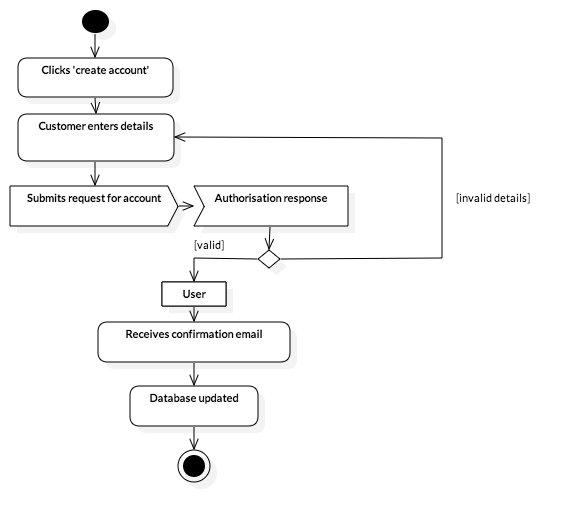
\includegraphics[trim = 0 0 0 0, clip, width=0.6\textwidth]{TempImg/newUserAD.png}
      \caption{Activity diagram for UC1: Creates Account}
 \end{figure}

\begin{figure}[H]
      \centering
      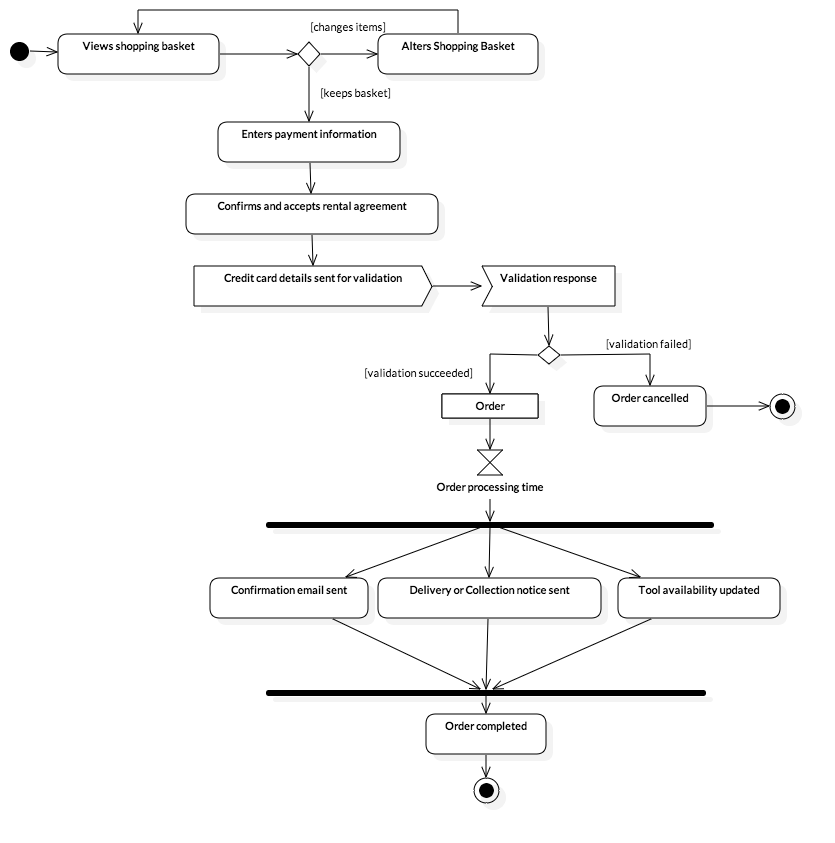
\includegraphics[trim = 0 0 0 0, clip, width=0.9\textwidth]{TempImg/checkoutAD.png}
      \caption{Activity diagram for UC8: Checks Out}
 \end{figure}

\begin{figure}[H]
      \centering
      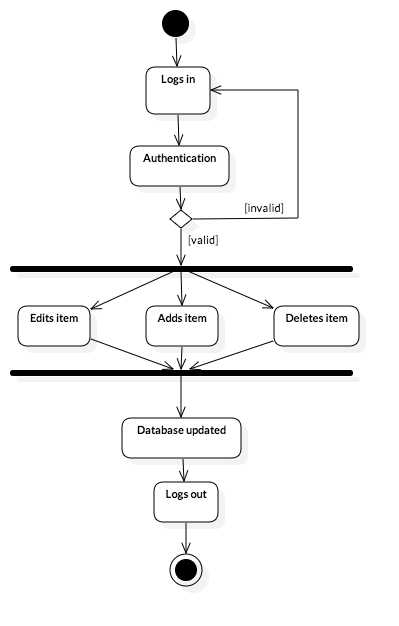
\includegraphics[trim = 0 0 0 0, clip, width=0.45\textwidth]{TempImg/manageToolsAD.png}
      \caption{Activity diagram for UC6: Manages Tool Listings}
 \end{figure}

\hypertarget{uml-class-diagrams}{%
\subsection{UML Class Diagrams}\label{uml-class-diagrams}}

\hypertarget{overview-2}{%
\subsubsection{Overview}\label{overview-2}}

With the functional requirements of the THS established and use cases
developed to model the user interaction with the system, it was
necessary to begin to move from the problem domain to the solution
domain and move more towards the language of the developer, structured
by classes and packages rather than use cases. {[}1{]}

In doing so, the domain model and use cases were analysed to identify
the key objects to be modelled in the system. With the objects
identified, the data attributes of the objects and method call sequences
required to realise the use cases were established through an iterative
process of role play and pseudo-code development. This resulted in an
analysis class diagram - showing the key objects and their
relationships, a design class diagram -- a more comprehensive and
defined representation of the system's classes, sequence and activity
diagrams, state machine diagrams and a deployment diagram, which will be
discussed in the following sections.

\hypertarget{analysis-dlass-diagram}{%
\subsubsection{Analysis Dlass Diagram}\label{analysis-dlass-diagram}}

A use-case driven approach was used to identify the key nouns and verbs
and iteratively develop these into the system's objects and method
calls. The analysis class diagram in Figure 4.6 shows a middle stage
iteration. The classes are labelled as either boundary, controller or
entity classes in line with the Jacobson categorisation style {[}10{]}.
In this style, the boundary classes encapsulate output data and
generates output in the required form, the controller classes deal with
controlling behaviour and completing tasks and the entities classes
store the data and define operations on the data. The advantage of this
is that it enforces clear partitioning of responsibilities in the class
structure early on in the object-oriented design process.

The class names were kept close to the functionality of the class which
will allow for clarity in the development phase. The relationships
(associations, generalisations, dependencies, aggregations and
compositions) were mapped between the classes only where a relationship
was necessary to achieve a use case.

\begin{figure}[H]
      \centering
      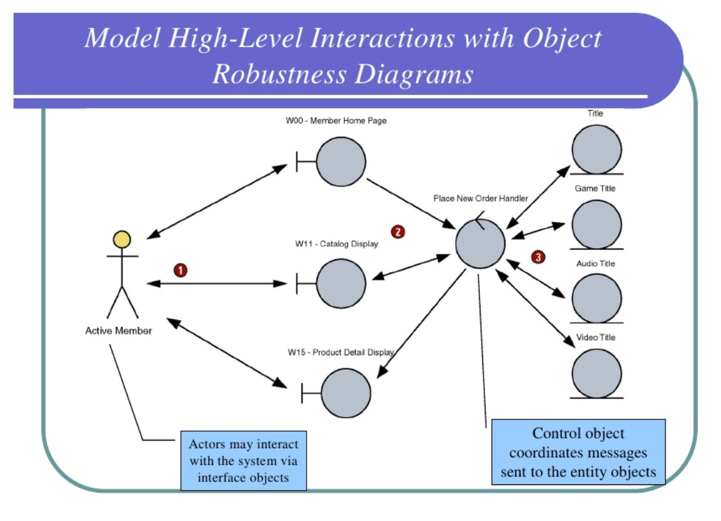
\includegraphics[trim = 0 0 0 0, clip, width=0.7\textwidth]{TempImg/OOClass.png}
      \caption{A model of Boundary-Control-Entity architecture [11]}
 \end{figure}

\begin{figure}[H]
      \centering
      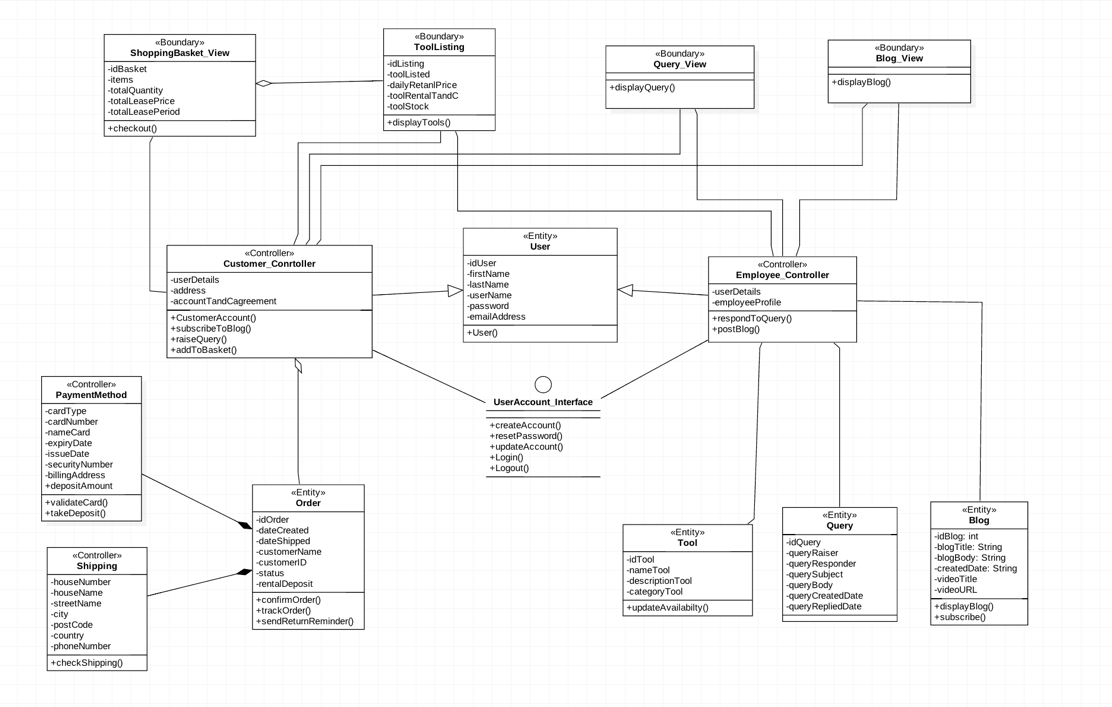
\includegraphics[trim = 0 0 0 0, clip, width=0.99\textwidth]{TempImg/AClass.png}
      \caption{Analysis Class Diagram}
 \end{figure}

\hypertarget{design-class-diagram}{%
\subsubsection{Design Class Diagram}\label{design-class-diagram}}

The analysis diagram was used as a basis to build the design class
diagram, which specifies in more detail how the system will be
implemented, getting closer to the solution domain. There was a strong
focus on adhering to object-oriented principles. Some of the
considerations that went into the design class diagram are discussed
here:

\hypertarget{adding-implementation-details}{%
\paragraph{Adding implementation
details}\label{adding-implementation-details}}

Variable types, method parameters and return types were added, along
with variable and method visibility. Adhering the object-oriented
principle of \textbf{encapsulation} most class member variables were
given private visibility with public methods that allow access to them.
(NB for the sake of coherence of the diagram, not all getters and setter
were modelled for every class).

\textbf{Static methods} were also used where there was no need for the
method to use instance variables and the method therefore belongs to the
class rather than an instance of the class. For example - the methods in
the database connector are static, as is the `connectionStatus'
variable. This makes the class a \textbf{singleton class} {[}12{]}
whereby only one instance of the class need exist in the Java Virtual
Machine and providing a global point of access to other classes that
need it.

\textbf{Inheritance} was used only where needed -- to generalise a
customer and employee to a user -- thereby eliminating duplication of
user details in each class. It was also used in the `PaymentMethod'
(parent) and `Deposit' (child) relationship.

\textbf{Interfaces} were used to help separate the specification of an
entity from implementation of a task. For example - the employee
controller manages a tool listing via a `manageToolListing' interface.
This has the advantage that in the future, should the GUI for the tool
listing change, it is easier to change the implementation of the `manage
tool listing' methods.

\hypertarget{completeness-primitiveness}{%
\paragraph{Completeness \&
Primitiveness}\label{completeness-primitiveness}}

\textbf{Completeness: } this is the specification that the design
classes should cover all the data and functionality needed. We ensured
this by iteratively mapping out use case flows and ensuring that classes
are related and can therefore access instances of each other when
required. Classes were also added from the analysis class where needed.

\textbf{Primitiveness:} this is the specification that there should
never be more than one way of doing things. For example -- in our system
there is just a single `respondToQuery()' method that encompasses
different types of query rather than several separate methods.

\hypertarget{high-cohesion-low-coupling}{%
\paragraph{High Cohesion \& Low
Coupling}\label{high-cohesion-low-coupling}}

\textbf{High cohesion: } this specifies that each class should model a
single abstract concept {[}9{]}. We ensured this by separating out the
implementation for managing queries/blog/tool listing/shopping
basket/user accounts -- so that the employee and customer controllers do
not take on several different responsibilities. This is also the case
for the database connector which is a simple class, just concerned with
connecting to the database, the create/read/update methods are present
in the respective entities.

\textbf{Low coupling: }This specifies that classes should associate with
just enough other classes to realise its goal -- e.g.~which was achieved
by using focused aggregation rather than inheritance in most places.

\begin{figure}[H]
      \centering
      \includegraphics[trim = 0 0 0 0, clip, width=0.89\textwidth]{TempImg/Dclass.png}
      \caption{Design Class Diagram}
 \end{figure}

\hypertarget{sequence-diagrams}{%
\subsection{Sequence Diagrams}\label{sequence-diagrams}}

Sequence diagrams serve as the bridge between use-cases and class
diagrams. They are a type of interaction diagram which describes the
order in which interactions in a system occur. The events in sequence
diagram are shown chronologically, with the earliest event at the top of
the diagram and the last event at the bottom. Events occur between
participants, which in the case of the THS, are actors, databases, and
classes derived from the class diagram. Each event has a message which
describes the interaction between participants. Methods from the design
class diagram are used as messages and allow the classes to interact.
Interactions between the actors and boundaries have messages given in
pseudo code to describe the real-world interaction between the user and
the interface. {[}9{]}

For the purposes of this project, messages were given without arguments.
Given that team determined that the diagrams were useful and adequately
descriptive using this high level approach, the arguments were
intentionally left out to reduce clutter. Six sequence diagrams are
given below to illustrate some of the most relevant use-cases in
addition to a key describing the features that appear. (Figure 4.9)

\begin{figure}[H]
      \centering
      \includegraphics[trim = 0 0 0 0, clip, width=0.6\textwidth]{TempImg/SDKey.png}
      \caption{Sequence diagram symbol key}
\end{figure}

\begin{figure}[H]
      \centering
      \includegraphics[trim = 0 0 0 0, clip, width=0.7\textwidth]{TempImg/add_new_tool_SD.png}
      \caption{Sequence diagram for adding a new tool listing to the THS system. This is a version of UC6: Manages Tool Listing}
\end{figure}

\begin{figure}[H]
      \centering
      \includegraphics[trim = 0 0 0 0, clip, width=0.7\textwidth]{TempImg/new_user_reg_SD.png}
      \caption{Sequence diagram for registering a new customer to the THS system. This is a version of UC1: Creates Account}
\end{figure}

\begin{figure}[H]
      \centering
      \includegraphics[trim = 0 0 0 0, clip, width=0.8\textwidth]{TempImg/create_order_SD.png}
      \caption{Sequence diagram for creating an order in the THS system. This is a version of UC7: Creates Order}
\end{figure}

\begin{figure}[H]
      \centering
      \includegraphics[trim = 0 0 0 0, clip, width=0.99\textwidth]{TempImg/check_out_SD.png}
      \caption{Sequence diagram for checking out. This is a version of UC8: Checks Out}
\end{figure}

\begin{figure}[H]
      \centering
      \includegraphics[trim = 0 0 0 0, clip, width=0.8\textwidth]{TempImg/make_blog_post_SD.png}
      \caption{Sequence diagram for an admin creating a blog post. This is a version of UC23: Posts Advice Blog & Video Tutorials}
\end{figure}

\begin{figure}[H]
      \centering
      \includegraphics[trim = 0 0 0 0, clip, width=0.8\textwidth]{TempImg/make_query_SD.png}
      \caption{Sequence diagram for a customer entering a query into the THS system. This is a version of UC19: Raises Query}
\end{figure}

\hypertarget{state-machine-diagram}{%
\subsection{State machine diagram}\label{state-machine-diagram}}

In this section three state machine diagrams are displayed and
explained.

\hypertarget{tool-rental-lifecycle}{%
\paragraph{Tool Rental Lifecycle}\label{tool-rental-lifecycle}}

This diagram represents the lifecycle of the tool hire from the
perspective of the tool itself. The tool can switch between four states
which are: \textit{Available, Booked, Serviced and Maintained}. The
lifecycle begins at the available state. After the tool is booked by a
client the tool changes its state to booked. Subsequently, once the tool
is returned it is checked on functionality and observable flaws.
Consequently, the tool is either serviced, if it needs repair or it is
put back in the state of maintained. After this last step, the tool is
ready for rental again and the state of the tool is changed to
available. This closed the cycle and the loop continues.

\begin{figure}[H]
      \centering
      \includegraphics[trim = 0 0 0 0, clip, width=0.8\textwidth]{TempImg/ToolSM.png}
      \caption{State machine diagram for a tool rental}
\end{figure}

\hypertarget{order}{%
\paragraph{Order}\label{order}}

This diagram visualises the five different states from the shipping
perspective. The five states are:
\textit{Pending, Packed, Dispatched, Delivered, Returned and Closed.}

Once the client completed his order, the order changes its state to
pending, after the shipping is initialized the state of the order is
changed to packed. Consequently, the ordered tool will be dispatched. If
the order could not be delivered, it will be returned and dispatched
again. Once the shipping is completed it will change its state to
delivered. As soon as the order is cleared the order will change to the
final state, which is the closed status.

\begin{figure}[H]
      \centering
      \includegraphics[trim = 0 0 0 0, clip, width=0.8\textwidth]{TempImg/OrderSM.png}
      \caption{State machine diagram for an order}
\end{figure}

\hypertarget{shopping-basket}{%
\paragraph{Shopping Basket}\label{shopping-basket}}

The following state machine diagrams displays the four stages of the
shopping basket. The four states are:
\textit{Empty, Collecting, Checked Out and Ordered.}

The initial state of the shopping basket is empty, once tools are added
it changes to the collecting state, if the added tool is deleted again
we find ourselves again in the empty state.In the collecting state,
arbitrarily many products can be added or deleted. As soon as 1 product
is in the basket, the collecting state is initialized. Once the client
confirms that the order the status is updated to checked out. If the
summary is accepted the shopping basket will convert to the final state
ordered. However, if the order is abandoned, the whole basket will be
cleared and it goes back to the initial state, empty.

\begin{figure}[H]
      \centering
      \includegraphics[trim = 0 0 0 0, clip, width=0.8\textwidth]{TempImg/BasketSM.png}
      \caption{State machine diagram for an order}
\end{figure}

\hypertarget{component-diagram}{%
\subsection{Component Diagram}\label{component-diagram}}

Figure 4.19 shows the component diagram, which indicates a static
representation of the projected system with interest to the logical
elements. This diagram represents part of the architectural features of
the system. It is more abstract, and it has less details than the
previous class and object diagrams, therefore, it helps to familiarize
with the system architecture. The DIY TOOL component diagram has four
fundamental but interconnected groups.

Groups of the components in the DIY Hire Service system:

\begin{itemize}
  \item Components related to the User interaction. It allows the users to interact with the system. We have a browser engine, that allow users to find the products; shopping basket, which manage client’s tools basket and the User Session, such as the log-in process.
  \item Components related to the Warehouse management. It manages which tools are available and in which quantity.
  \item Components related to the Payment System. It interacts with the APIs of several third-party payment services, such as Visa, MasterCard, PayPal. It allows to complete the transaction
  \item Components related to the Administration control. It controls the Orders flow and consequentially it depends on the other components. 
\end{itemize}

Each of the above stated groups includes of components of various types
such as: executables, libraries, files, ports, connectors and
interfaces. The figure below shows the components diagram which complies
with UML 2.0 notation standard.

\begin{figure}[H]
      \centering
      \includegraphics[trim = 0 0 0 0, clip, width=0.9\textwidth]{TempImg/compD.png}
      \caption{System components diagram}
\end{figure}

\hypertarget{three-tier-architecture}{%
\subsection{Three Tier Architecture}\label{three-tier-architecture}}

A three tier model partitions a system's component's into three layers
of services. These are more a representation of the logical tiers in a
system as opposed to a direct physical representation.

The outermost tier that us responsible for user interaction with the
system is called the presentation tier. {[}13{]} For the Tool Hire
Service, this means the website's interface with which the user
interacts. Through the use of Dynamic HTML a THS customer or employee
can interact with the services in the second tier in a simple and
intuitive manner. The second tier is known as the Logic or business
services layer. The processes contained in the second tier carry out the
actual logic and functionality of the application and have access to the
third tier. Since many clients can access this tier from different
devices simultaneously, it is important that this tier manages its
transactions in order to keep the data structures in the third tier
consistent and reliable. {[}14{]} An example of how this may be used in
the THS system would be if multiple customers were trying to book a tool
at the same time. The logic tier must be able to ``decide'' which
customer will get to rent the tool, update the database, and send a
message to each customer indicated the result. Managing such conflicts
in the second tier greatly reduces the burden on the third tier
services. {[}13{]}

Finally, the third and innermost tier comprises of a system's data. The
database management system (DBMS) and the data it manages can only be
accessed via the second tier. {[}13{]} This is where all data for the
system is stored. In the case of the THS, some example of data stored
here would be Order data, Customer data and Tool data. Access to this
layer can be seen in the design class diagram as the DBConnector class.

\begin{figure}[H]
      \centering
      \includegraphics[trim = 0 0 0 0, clip, width=0.9\textwidth]{TempImg/3TA.png}
      \caption{Three tiers for the THS system}
\end{figure}

Even though this architecture is more complex than a single tier, the
benefits of using a three tier architecture outweigh the drawbacks. The
three most important reasons a three tier architecture is suitable for
the THS are:

\begin{itemize}
  \item If the THS were to expand, the system is easily scalable since the data layer is independent from the other two.

  \item It is easier to maintain and modify the underlying code of the system if it is divided into separate layers, for example the UI can change without modifying the logic layer.

  \item Increased security with security defined for each layer. Since users can only access the second tier and not the third, if proper security measure are taken, a three tier architecture is more secure than a two tier architecture. However, having an additional tier means that during system development, security measure must be carefully discussed between developers working of different tiers in order to ensure that increased surface area doesn’t lead to increased risk. 

\end{itemize}

\hypertarget{deployment-diagram}{%
\subsection{Deployment Diagram}\label{deployment-diagram}}

The Deployment Diagram shown in Figure 4.21 shows the deployment of
various software artefacts generated by the Tool Hire Service (THS) to
deployment targets. Deployment targets are called nodes and can
represent a device such as a computer or a software execution
environment. The deployment diagram shows the full hardware architecture
of the THS. Included is the customer's desktop, a webserver, an
application server and finally a database. The customer's pc connects to
the web server where the website is hosted via HTTP (Hypertext Transfer
Protocol). The web server then connects to the application server via
RMI (Remote Method Invocation) which handles the business logic for
components such as orders, shipping and blog posts. Lastly the
application server connects to the database via JDBC (Java database
connectivity).

\begin{figure}[H]
      \centering
      \includegraphics[trim = 0 0 0 0, clip, width=0.6\textwidth]{TempImg/depD.png}
      \caption{Deployment diagram}
\end{figure}



\newpage

\hypertarget{application-mock-up}{%
\section{Application Mock-up}\label{application-mock-up}}

\hypertarget{user-manual}{%
\subsection{User Manual}\label{user-manual}}

Content Content Content Content Content Content Content Content Content
Content Content Content Content Content Content Content Content Content
Content Content Content Content Content Content Content Content Content
Content Content Content Content Content Content Content Content Content
Content Content Content Content Content Content

\begin{enumerate}

\tightlist
\item
  About 1
\item
  About 2
\item
  About 3
\end{enumerate}

\hypertarget{user-manual-2}{%
\subsubsection{User Manual 2}\label{user-manual-2}}

Content Content Content Content Content Content Content Content Content
Content Content Content Content Content Content Content Content Content
Content Content Content Content Content Content Content Content Content
Content Content Content Content Content Content Content Content Content
Content Content Content Content Content Content

\newpage

\hypertarget{conclusion}{%
\section{Conclusion}\label{conclusion}}

In this chapter, an overview will be provided of the utilized strategy
in order to give insights into the approach of the creation of the THS
system. The team met on a weekly basis and , To increase the
productivity, the team was divided into sub-groups to carry out varying
work simultaneously and efficiently. During the weekly group discussion,
the sub-groups results were reviewed by all the team members with an
open discussion in order to achieve high quality and consistency between
all members. The team worked in a reliable manner and internal deadlines
were met. The weekly progress was monitored by the team's advisor who
gave feedback and advice for the tasks for the following week..

The development approach was based on strong requirements and use cases.
The declaration of actors and their functionalities helped to create the
classes and methods required for the Object-Oriented Analysis stage. As
the team wanted to ensure that the flow of use cases was represented
properly, many iterations of object oriented diagrams were made. (See
Appendix) Although a lot of time was spent on reviewing the diagrams,
future iterations are possible in the development, which should be in
line with the tenants of the Unified Process.

The team has developed the project according to the standardised
documentation of the Unified Modelling Language (UML) and the process
has been created with an Object Oriented approach to the Analysis and
Design of a prototype version of the DIY tool renting website.

Great communication and well coordinated teamwork could be observed
throughout the duration of the course. Both internal and external
deadlines were met. Although the team met the weekly deadlines and
worked well, there were aspects that could be considered to be done
differently for future projects. There have been several difficulties to
synchronize the writing style between sections completed by different
people. To minimize this, there were regular reviews on each member's
contribution in order to ensure consistency.

\newpage

\hypertarget{references}{%
\section{References}\label{references}}

\begin{enumerate}
  \item Jacobson, G. Booch, J. Rumbaugh, The Unified Software Development Process, Addison-Wesley, 1999.
  \item J. Arlow and I. Neustadt, UML and the Unified Process. London: Pearson Education, 2002.
  \item K. Schwaber and J. Sutherland, "The Scrum Guide", scrumguides.org, 2017. 
  \item "What's the Difference? Agile vs Scrum vs Waterfall vs Kanban", www.smartsheet.com, 2018. 
  \item F. Brooks, The Mythical Man Month, Addison-Wesley, 1975.
  \item A. Kline, Agile Development in the Real World, Apress, 2015.  
  \item S. Ambler, Agile Model-Driven Development with UML 2.0, Cambridge University Press, 2004.
  \item A. Cockburn, Writing Effective Use Cases, the Crystal Collection for Software Professionals, Addison-Wesley, 2000.
  \item R. Miles & K.Hamilton, Learning UML 2.0, O’Reilly, 2006.
  \item A. Kalmback (2015). ‘Entity-Boundary-Interactor; A modern application architecture’. readthedocs.io [Online]. Available: http://ebi.readthedocs.io/en/latest/
  \item Whitten, L. Bentley and K. Dittman, Systems analysis and design methods. Boston, Mass.: Irwin/McGraw-Hill, 1998.
  \item E. Gamma, R. Helm, R. Johnson and J. Vlissides, Design patterns. Boston, Mass.: Addison-Wesley, 2016.
  \item "Three-tier architectures", ibm.com, 2018.
  \item “Using a Three-Tier Architecture Model", msdn.microsoft.com, 2018. 
\end{enumerate}
% -----------------------------------------------------------------------------------
%                               BIBLIOGRAPHY - Insert Name of BIB File Here
% -----------------------------------------------------------------------------------
\newpage

% ---------------BIBTEX OLD-----------------------------------------------------
% \bibliographystyle{unsrt} %%%% Plain or alpha can change orders here
% \bibliography{BibFile}
% \nocite{*} %%%if you want to see all references even those note cited in the text
% -----------------------------------------------------------------------------------

\printbibliography
% -----------------------------------------------------------------------------------
%                                  APENDIX
% -----------------------------------------------------------------------------------

% \end{counted} %<<<<<<<<<<<<<<ENDS WORD COUNTER

\newpage
\section{Appendices}

\subsection{Meeting Minutes}

\textbf{Meeting 1: 23rd Jan 2018}

Work Flow:

List of tasks for next 3 weeks compiled:

\textbf{Week 1:} Requirements gathering

\begin{itemize}
  \item Industry Research
  \item Everybody to research how to use Latex
  \item Shared resources to be set up: Github, Latex, One Drive

\end{itemize}


\textbf{Week2:} Refinement of requirements (including categorisation)

\begin{itemize}
  \item MoSCoW prioritisation and effort estimation for requirements
  \item Begin thinking about use cases


\end{itemize}


\textbf{Week 3:} Continue developing use cases

\begin{itemize}
  \item Need to consider who stakeholders for the app are (company, renters of tools).
  \item The application should be designed as a web app – for use in a browser and mobile.
  \item Phoebe to share UML 2.0 book to use for UML syntax / diagrams.
  \item Daiana to act as SCRUM master for project.


\end{itemize}


\textbf{Plan for next meeting}

To meet every Tuesday 11am - 1pm, possibly in room in Foster Court.

Next Meeting to bring post-its (!) to help organise requirements visually.

\textbf{Meeting 2: 30th Jan 2018}



\begin{itemize}
  \item This week focus on use cases and organise requirements.
  \item Brief discussions of Object oriented diagrams, sequence diagrams, activity diagrams
  \item Came up with non-functional requirements for the project
  \item Came up with non-functional requirements for the project
 
\end{itemize}



\textbf{First Meeting with Rae}

Review of vision and scope

Suggested we should convert requirements to excel and number them

She suggested that performance tests run on key functions can help determine non-functional requirements in an actual implementation

\textbf{Meeting 3: 6th Feb 2018}

\textbf{Discussed:}
Actors:

User – anyone that interacts with the system, Customer, Employee, Admin, Customer Support, Credit Card Company, Delivery service, Notification Service, Database

To Do this Week:
\begin{itemize}
  \item Finish writing up Use Cases and make sure they match names on use case diagram
  \item Finish analysis class diagram

\end{itemize}

\textbf{Meeting 4: 13th Feb 2018}

\begin{itemize}
  \item Refining Use-cases
  \item Discussion about state machine diagrams- Rae gave some examples and the group plans to review these
  \item Class diagrams- inclusion of getters and setters
  \item Sequence diagrams- making sure they are consistent with class diagrams


\end{itemize}

\textbf{Meeting 5: 6th March 2018}

\begin{itemize}
	\item Discussion of analysis and design class diagrams final changes- adding JSP/JavaClass notation to design and Boundary, Controller, Entity notation to the analysis class diagrams
	\item Discussion of final modification for sequence diagrams
	\item Clarification about deployment diagrams- modelling how a three tier architecture system would be deployed

\end{itemize}

\textbf{Meeting 6: 15th March 2018}

\begin{itemize}
	\item Final diagrams discussed 
	\item Discussion of report section allocation
	\item Discussion of presentation assembly

\end{itemize}




\subsubsection{Appendix 1 subsection}

\begin{enumerate}

  \item one
  \item two
  \item three
  \item four

\end{enumerate}


\subsection{Appendix 2}

\subsection{Appendix 3}






\end{document}